
\chapter{Transport of energy by radiation and conduction.}
\PartialToc

\section{Radiative transfer}

Photons emitted thermally in hotter regions and absorbed in cooler transfer energy. The effectiveness depends on thermal gradient and ability of the photons to travel freely (among others).The rate of radiative energy transport will be proportional to gradient of fourth power of T.

The reduction of intensity of a beam of photons passing through matter is
\begin{align*}
&\TDy{x}{I}=-\overline{\kappa}\rho I\\
&dI_{\nu}=-\kappa_{\nu}\rho I_{\nu}\,ds
\end{align*}



\subsection{Absorption/scattering coefficients}

$\kappa_{\nu}$ is the mass absorption coefficient: it includes processes of absorption and scattering. In star's interior where matter is completely ionized the bulk of scattering occurs from Thomson scattering by free electrons whereas in cool atmosphere may be due to molecular scattering.

\begin{align*}
&dI_{\nu}=-\kappa_{\nu a}\rho I_{\nu}\,ds\\
&dI_{\nu}=-\kappa_{\nu s}\rho I_{\nu}\,ds\int_{\Omega'}p(\cos{\theta'})\frac{d\Omega'}{4\pi}
\end{align*}
$p(\cos{\theta'})$ is the scattering phase function which gives angular distribution of scattered energy removed from the beam: for Rayleigh scattering $p(\cos{\theta'})=1+\cos^2{\theta'}$.

\subsection{Emission of photons: kirchhoff law}

$j_{\nu}(\theta)$ represents the true emission of radiation of freq. $\nu$ per unit frequency interval in direction $\theta$ per unit solid angle from each gram of stellar matter. The specific intensity of radiation at angle $\theta$ will be increased by

\begin{align*}
&dI_{\nu}(\theta)=j_{\nu }\rho\,ds&\intertext{assumption that stellar interior is in local thermodynamic equilibrium: matter radiates spontaneously in stellar interior as it would in thermodynamic equilibrium: stellar matter is assumed to have temperature T and assumption of local thermodynamic equilibrium is that matter at T radiates exactly as it would if it were in surroundings in thermodynamic equilibrium at same T  :}\\
&I(\theta)=\frac{c}{4\pi}u\ (+\frac{3}{3\pi}H\cos{\theta})&\intertext{sine T gradient is small compared to mean free path of photns in stellar interior the photons are absorbed at same temperature they are emitted. Condition for LTE:}\\
&j_{\nu}=\kappa_{\nu a}\frac{cu_{\nu}}{4\pi}=\kappa_{\nu a}B_{\nu}(T)&\intertext{kirchhoff law}
\end{align*}

Part of the emissions contained in kirchhoff law is spontaneous emission resulting only from T and part is induced emission. The induced emission comes from atomic transitions caused by radiation field and produes radiation with same freq. and moving in same pencil of direction as incident radiation.

\begin{usefull}{Fraction of total emission that is spontaneous}

\begin{align*}
&\frac{\text{Spontaneous}}{\text{Total}}=\frac{N_iA_{ij}}{N_iA_{ij}+N_iB_{ij}u_{\nu_{ij}}}\\
&=\frac{1}{1+(B_{ij}/A_{ij})u_{\nu_{ij}}}
&\intertext{where $\frac{1}{4\pi}N_iA_{ij}$ is a spontaneous transition rate per unit solid angle, $\frac{1}{4\pi}N_iB_{ij}u_{\nu_{ij}}$ is the rate of photons emission (in same direction of incident photons) per unit solid angle, induced by encounters of atoms in state i with photons $\nu_{ij}$}\\
&\frac{\text{Spontaneous}}{\text{Total}}=1-\exp{-\frac{h\nu}{kT}}&\intu{Qm radiation theory requires that this ratio of spontaneous to total emission in local thermodynamic equilibrium apply to any mechanism of true absorption}
\end{align*}

there are mechanism other than transitions between atomic states that represent true emission/absorption: ionization is a true absorption, whereas inverse process is true emission.

\begin{definition}{Induced ionization/recombination}
QM can be show that radiative recombination of ion and electrons with emission of a photon $\nu_{ij}$ can be induced by presence of second photon $\nu_{ij}$.
\end{definition}

One reaches a ratio of spontaneous emission for radiative recombination to total emission by radiative recombination equal to that for atomic transitions.



\end{usefull}

\subsection{Slightly anisotropic radiation field in stellar interior}

One must be cautious to avoid making a mistake in extending properties of radiation computed for condition of local thermodynamic equilibrium to slightly anisotropic radiation field in stellar interior.

If deviation from strict thermodynamic equilibrium occur emission must be separated into two terms: spontaneous emission is still determined by T of matter and the source function is $B_{\nu}(T)$ whereas the induced emission is proportional to actual specific intensity of radiation $I_{\nu}(\theta)$ instead of $B_{\nu}(T)$:
\begin{equation*}
j_{\nu}(\theta)=\kappa_{\nu a}(1-\exp{-\frac{h\nu}{kT}})B_{\nu}(T)+\kappa_{\nu a}\exp{-\frac{h\nu}{kT}}I_{\nu}(\theta)
\end{equation*}

\subsection{Energy introduced into pencil by scattered photons}

Energy scattered per unit solid angle into pencil moving in direction $(\theta,\phi)$ from a pencil in direction $(\theta',\phi')$:
\begin{equation*}
j_{\nu,scat}=\kappa_{\nu s}\frac{1}{4\pi}\int_0^{\pi}\int_0^{2\pi}p(\theta,\phi,\theta',\phi')I_{\nu}(\theta',\phi')\sin{\theta'}\,d\theta'\,d\phi'
\end{equation*}

\subsection{Energy balance: equation of transfer}

We consider a cylinder with axis along $(\theta,\phi)$
\begin{align*}
&\Dcvar{\TDy{t}{Q}}{top}=-I_{\nu}(r+dr,\theta)\,d\Omega&\intu{power exiting from top}\\
&\Dcvar{\TDy{t}{Q}}{bot}=I_{\nu}(r,\theta)\,d\Omega&\intu{power entering from bottom}\\
&\Dcvar{\TDy{t}{Q}}{abs}=-(\kappa_{\nu a}+\kappa_{\nu s})\rho I_{\nu}(r,\theta)\,dl\,d\Omega&\intu{power per unit area absorbed during transit of cylinder}\\
&\Dcvar{\TDy{t}{Q}}{emis}=\kappa_{\nu a}\rho\,dl[(1-\exp{-\frac{h\nu}{kT}})B_{\nu}(T)\\
&+\exp{-\frac{h\nu}{kT}}I_{\nu}(\theta)]\,d\Omega+\kappa_{\nu s}\rho\,dl\frac{d\Omega}{4\pi}*\\
&\iint p(\theta,\phi,\theta',\phi')I_{\nu}(r,\theta',\phi')\sin{\theta'}\,d\theta'\,d\phi'
\end{align*}

From energy conservation \mblock{\Dcvar{\TDy{t}{Q}}{tot}=0}:

\begin{align*}
&I_{\nu}(r+dr,\theta)-I_{\nu}(r,\theta)=\PDy{r}{I_{\nu}}\,dr=\\
&-(\kappa_{\nu a}+\kappa_{\nu s})\rho I_{\nu}(r,\theta)\,dl\\
&+(1-\exp{-\frac{h\nu}{kT}})B_{\nu}(T)\kappa_{\nu a}\rho\,dl\\
&+\exp{-\frac{h\nu}{kT}}I_{\nu}(\theta)\kappa_{\nu a}\rho\,dl\\
&+\kappa_{\nu s}\frac{\rho\,dl}{4\pi}*\int p(\theta,\phi,\theta',\phi')I_{\nu}(r,\theta',\phi')\,d\Omega'
\end{align*}

Using \mblock{dr/dl=\cos{\theta}} and \mblock{\kappa_{\nu a}^*=\kappa_{\nu a}(1-\exp{-\frac{h\nu}{kT}})}:

\begin{align*}
&\frac{1}{\rho\,dl}\PDy{r}{I_{\nu}}\,dr=\frac{1}{\rho}\PDy{r}{I_{\nu}}\cos{\theta}\\
&=-(\kappa_{\nu a}^*+\kappa_{\nu s})I_{\nu}(r,\theta)+\kappa_{\nu a}^*B_{\nu}(T)\\
&+\kappa_{\nu s}\frac{1}{4\pi}*\int p(\theta,\phi,\theta',\phi')I_{\nu}(r,\theta',\phi')\,d\Omega'
\end{align*}

It's the desired equation of radiative transfer for plane parallel atmosphereunder LTE.

\subsection{Photon gas}

Assuming polar axis parallel to direction of net flow.

\begin{align*}
&P_r=\frac{1}{3}\intzi{}\frac{h\nu}{c}cn(\nu)\,d\nu\\
&I(\theta)\,d\Omega=cu(\theta)\,d\Omega&\intu{$u(\theta)\,d\Omega$ represent energy density of radiation moving at angle $\theta$ in $d\Omega$}\\
&H=\int\,d\Omega I(\theta)\cos{\theta}&\intertext{stellar radiation is anisotropic in radial direction}\\
&I(\theta)\approx\frac{c}{4\pi}u+\frac{3}{4\pi}H\cos{\theta}+\ldots&\intu{the second term is much smaller than the first}
\end{align*}

\begin{figure}[!ht]
\centering
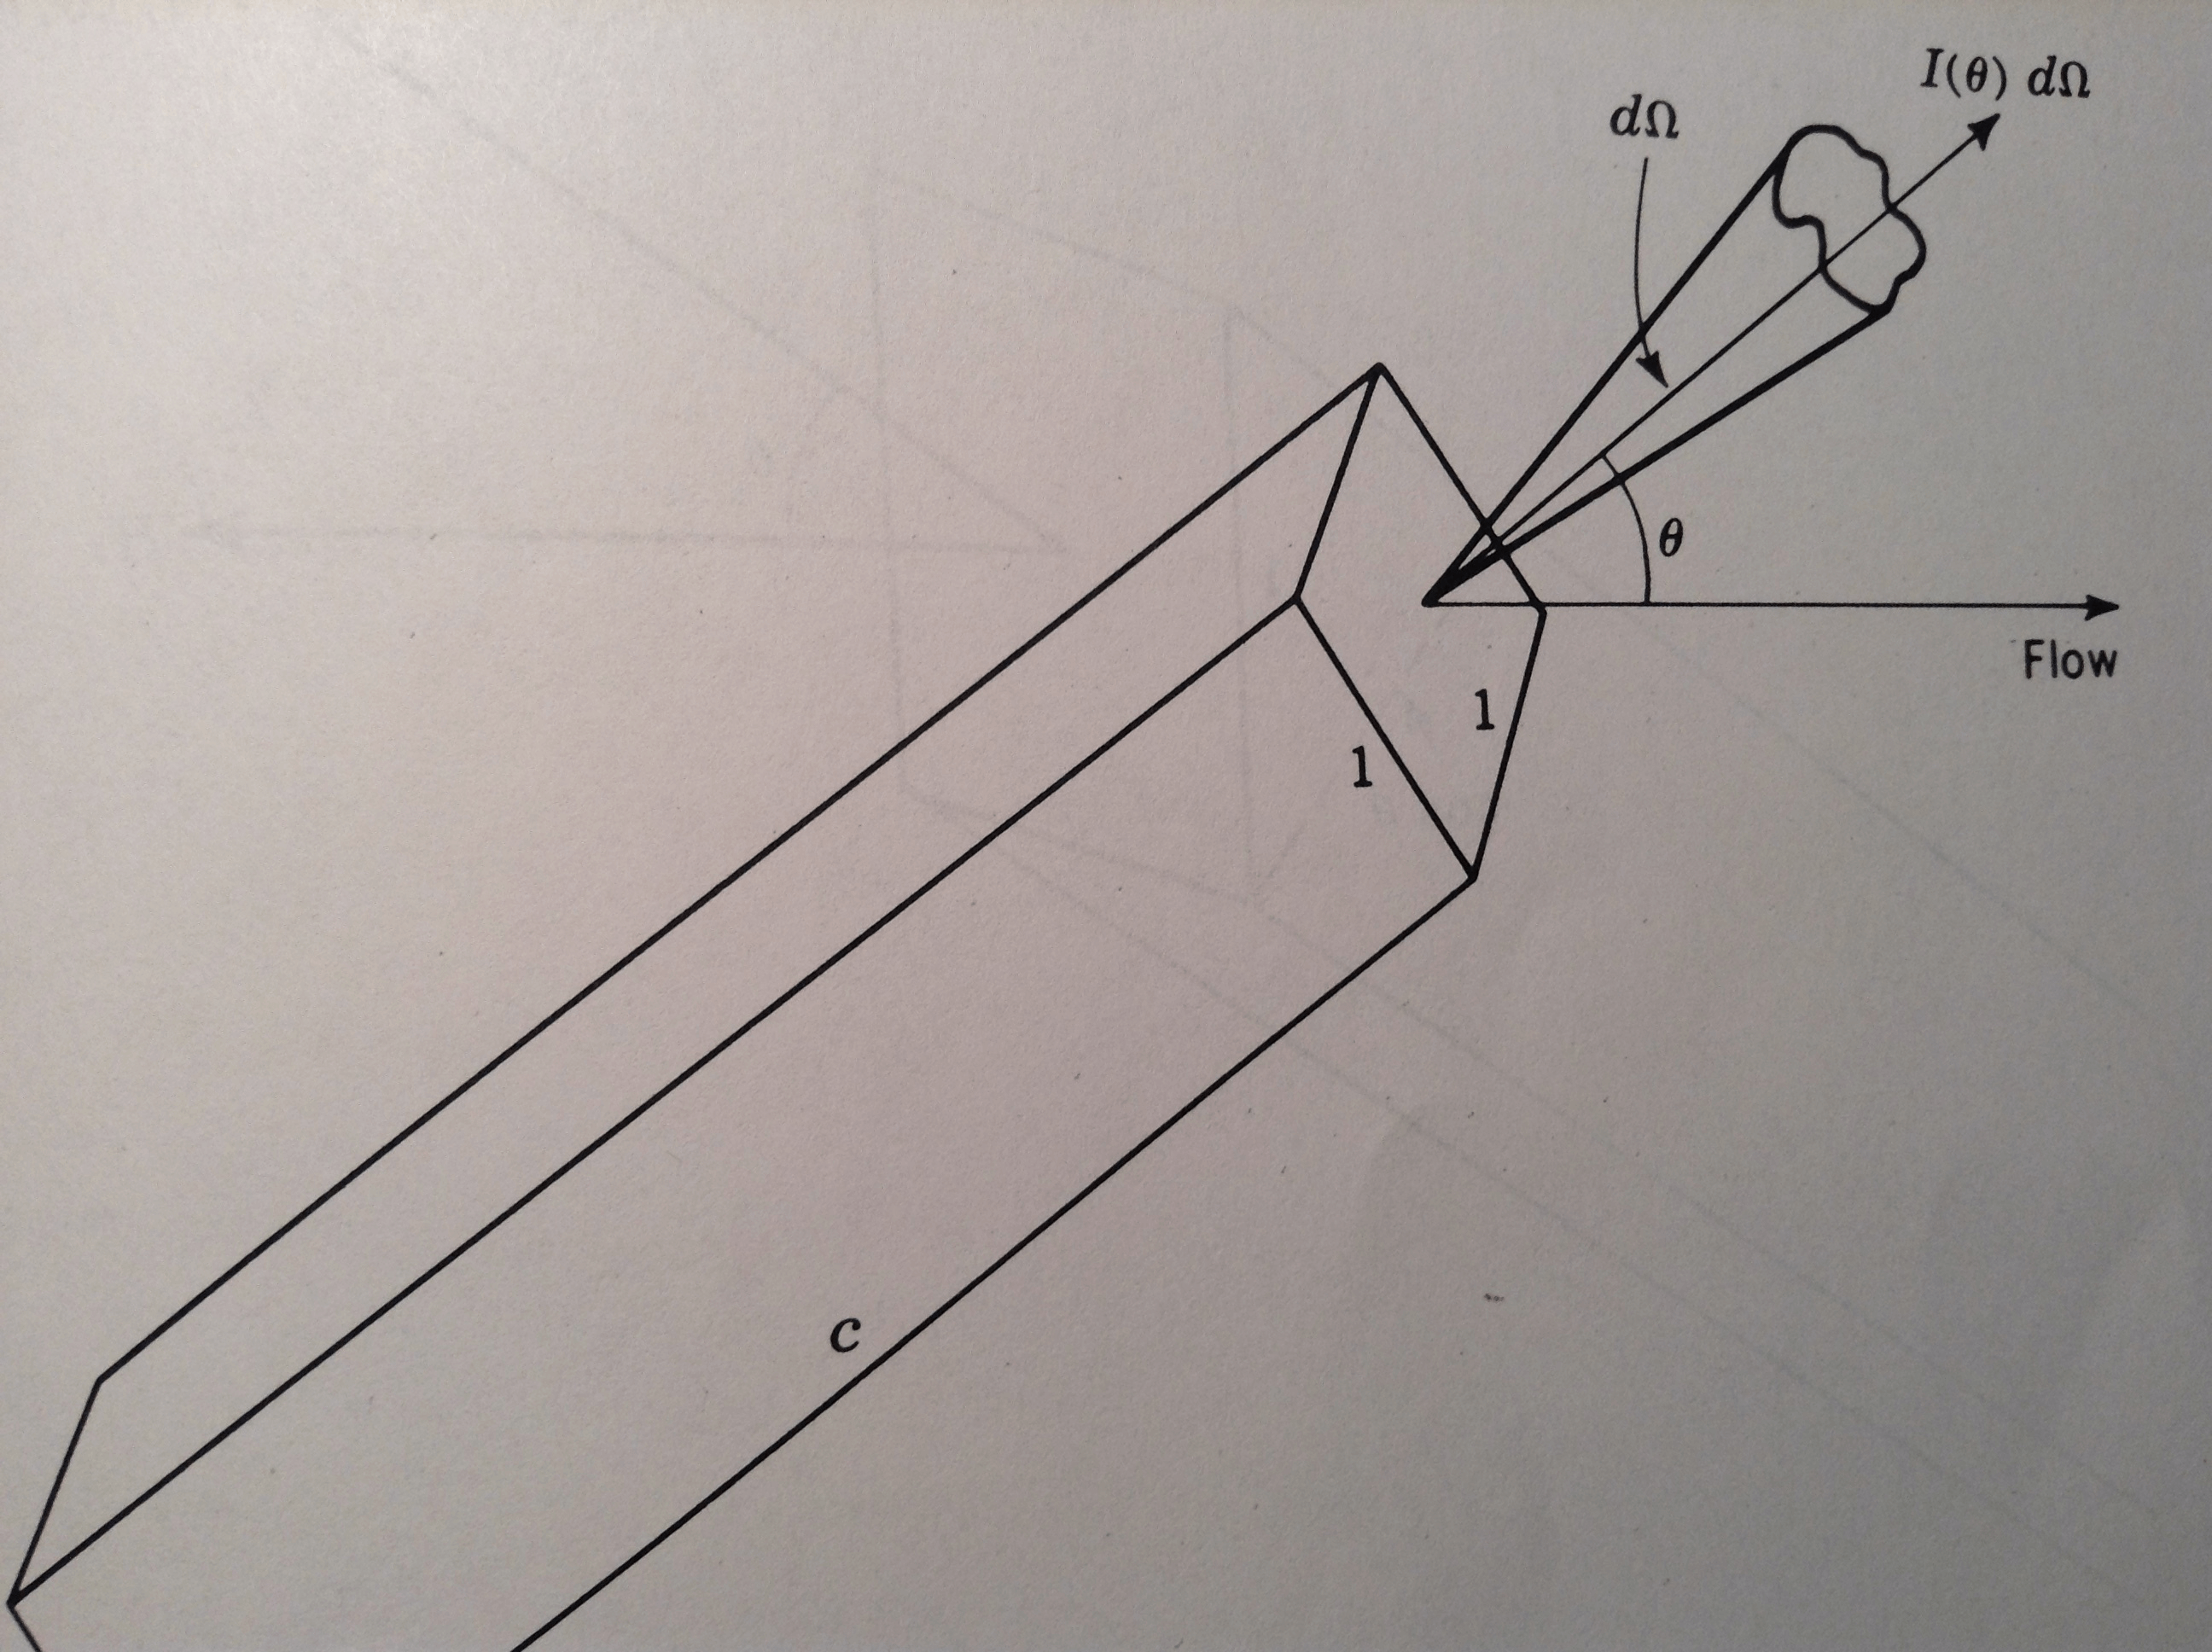
\includegraphics[width=\textwidth,height=0.9\textheight,keepaspectratio]{intensity}
\caption{$I(\theta)\,d\Omega$ is the energy flux moving in direction $\theta$}\label{fig:energyflux}
\end{figure}

\begin{figure}[!ht]
\centering
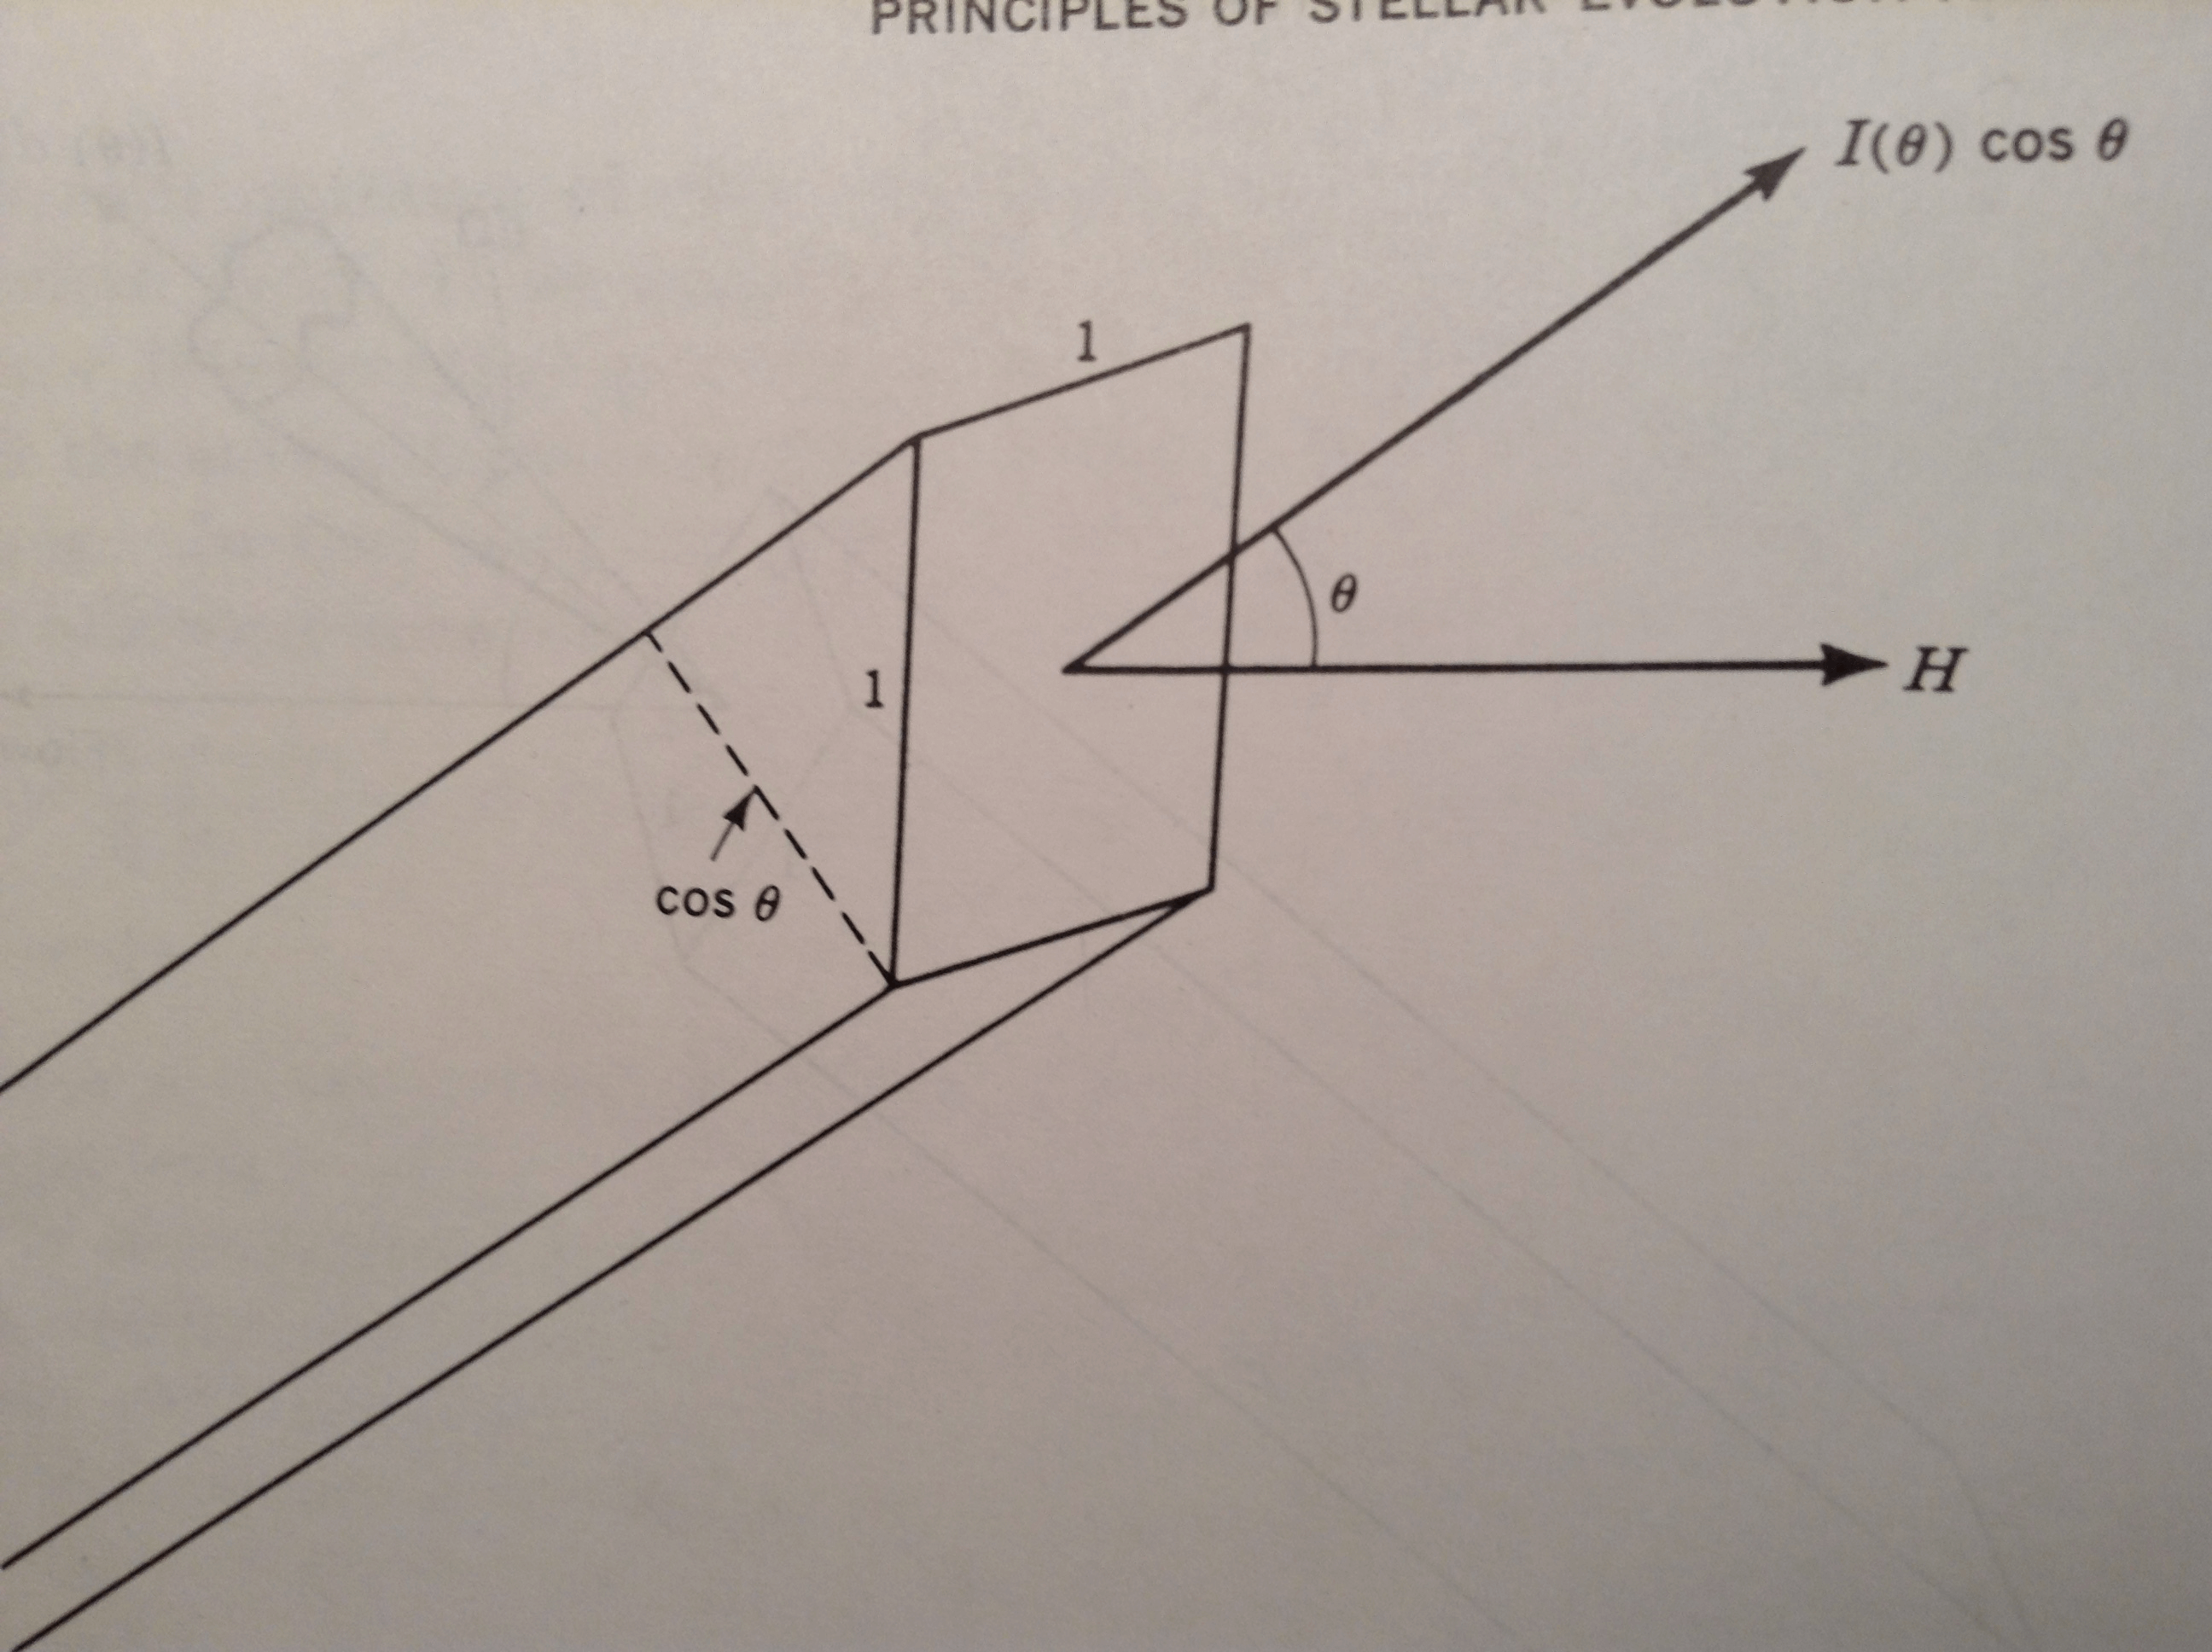
\includegraphics[width=\textwidth,height=0.9\textheight,keepaspectratio]{flux}
\caption{Energy flux with $I(\theta)\,d\Omega$ with associated energy flow per unit area normal to polar axis H equals to $I(\theta)\,d\Omega\cos{\theta}$.}\label{fig:energyflux}
\end{figure}

\begin{figure}[!ht]
\centering
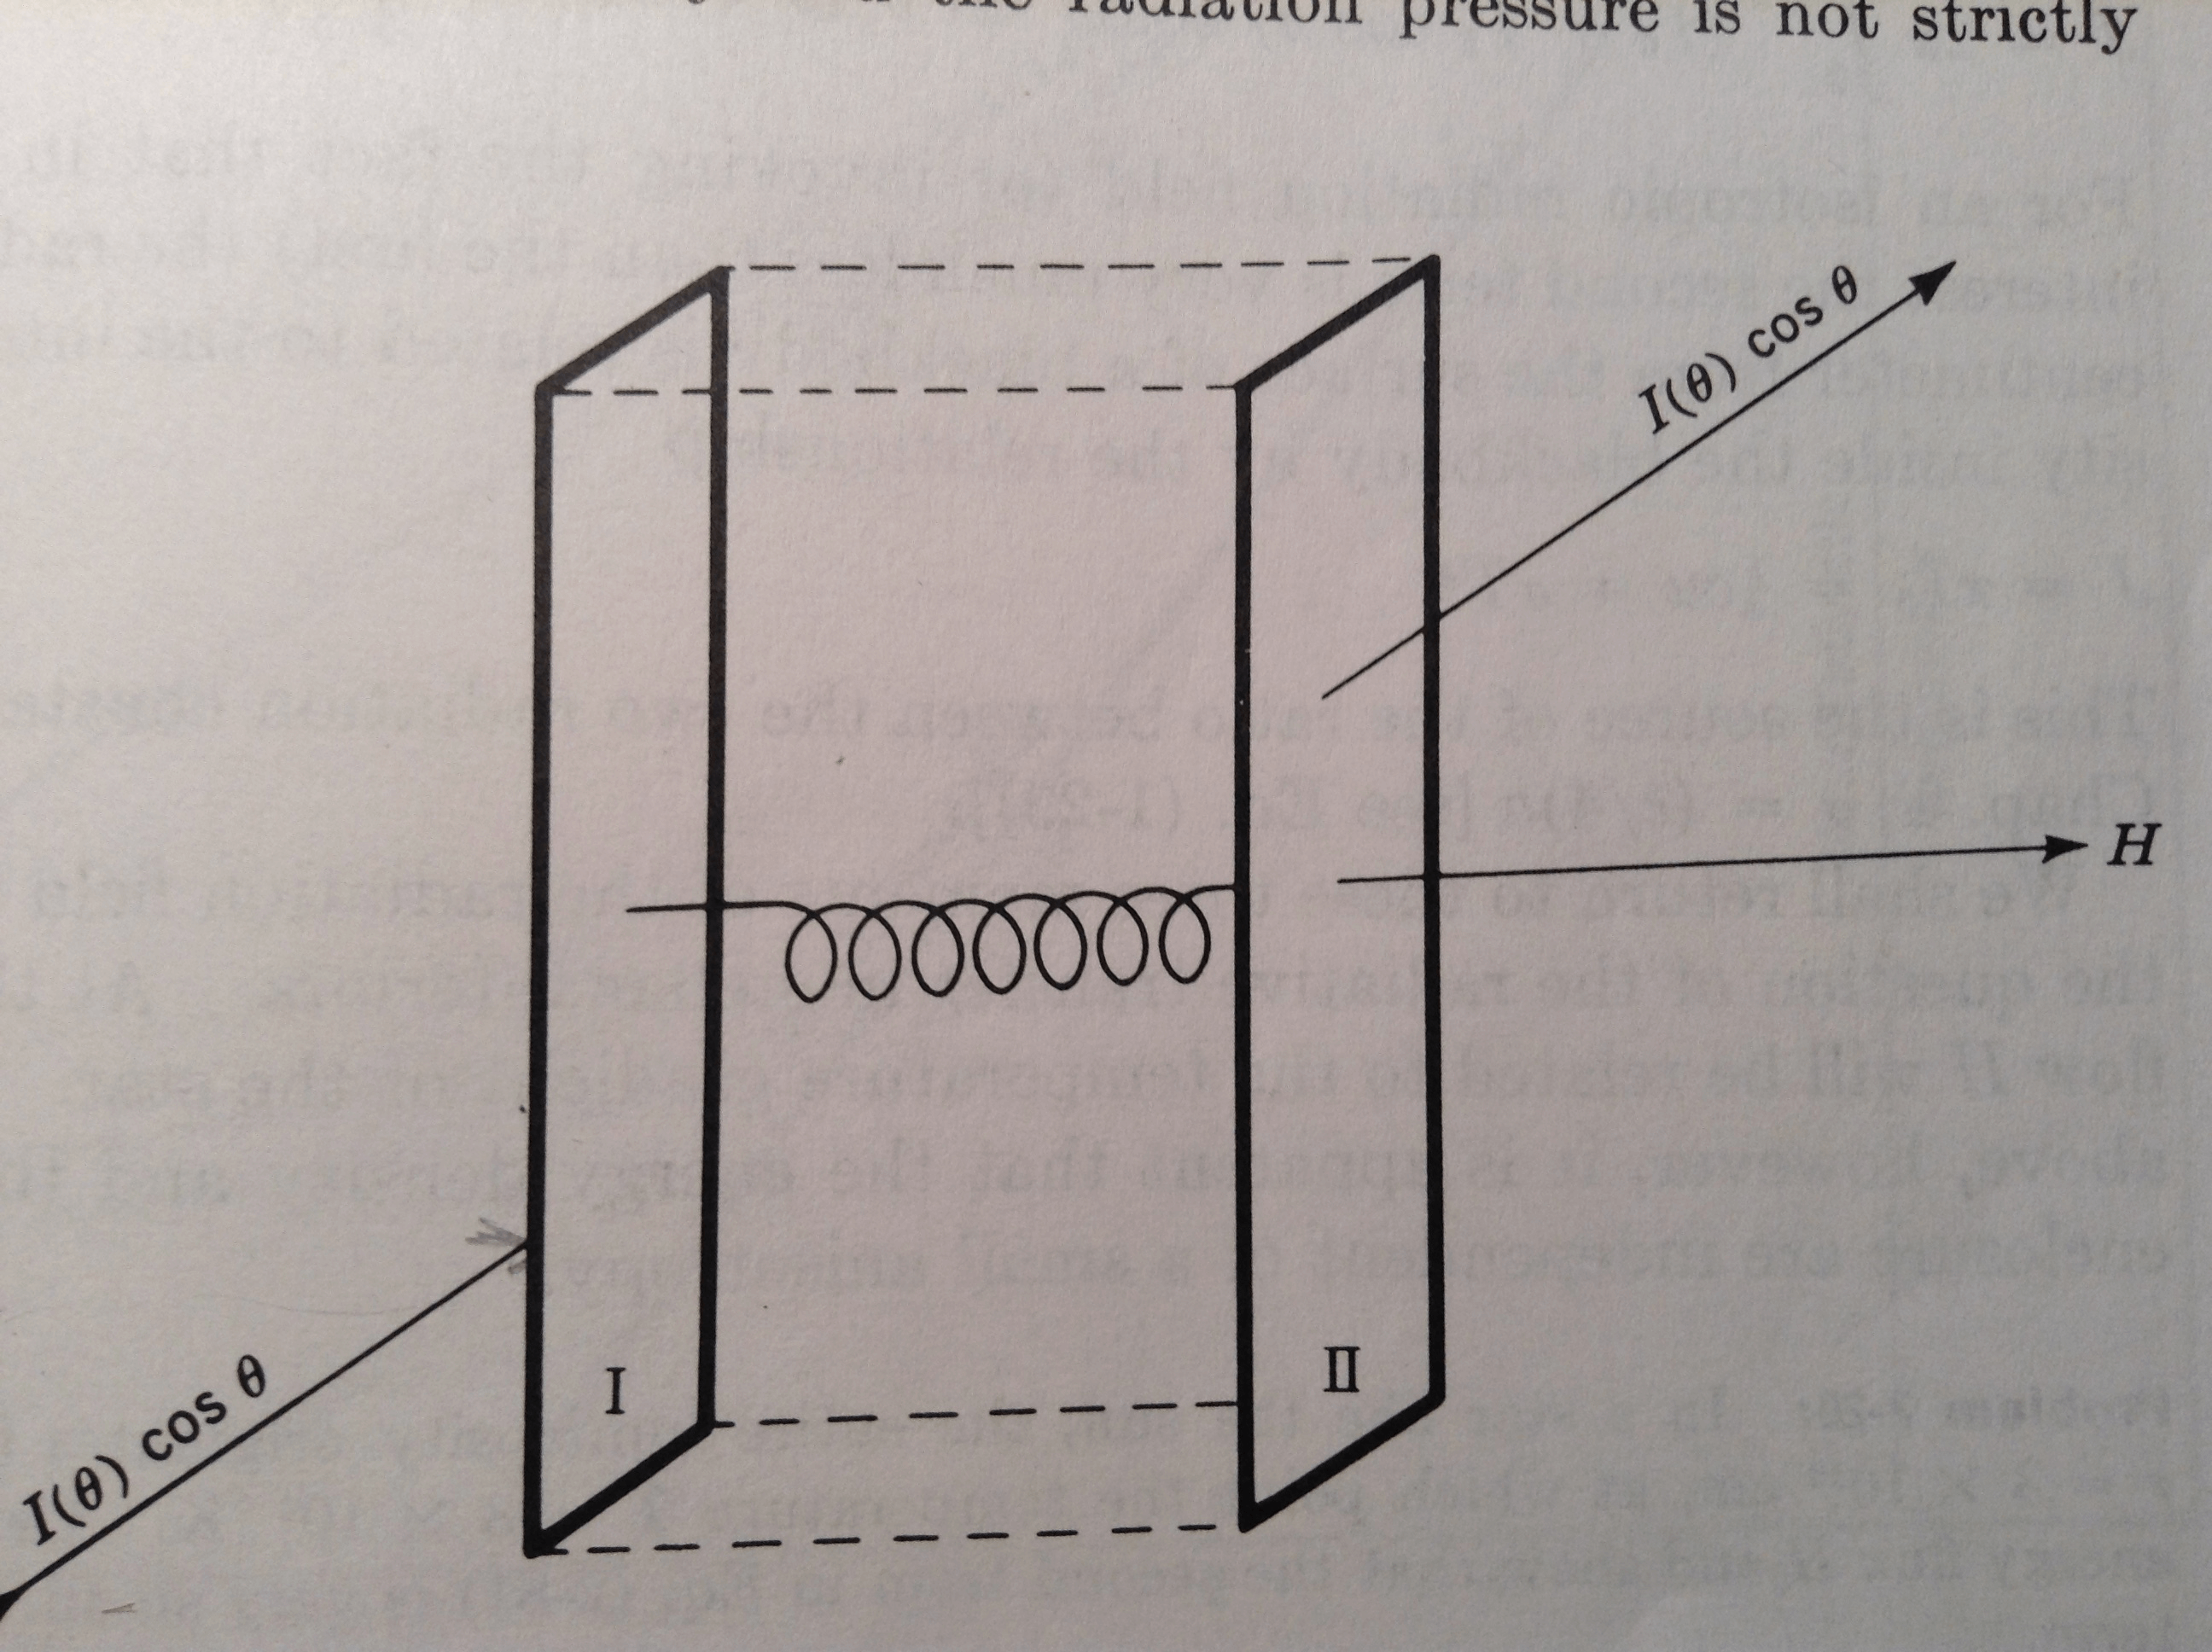
\includegraphics[width=\textwidth,height=0.9\textheight,keepaspectratio]{radpres}
\caption{The radiation pressure is the resulting compressional force on the spring.}\label{fig:radpressure}
\end{figure}

\clearpage

\subsection{Energy flow per unit area in terms opacity and temperature gradient}

\begin{usefull}{A quantity per unit dimension}
Describe characteristic properties of a unitary dimensional entity: mass of unitary surface base cylinder is $\rho\,dl$.
\end{usefull}

What is desired for computation of stellar structure is an equation of transfer that gives energy flow per unit area in terms of an averaged opacity and temperature gradient.

Multiplying the radiative equation transport by $\cos{\theta}$ and dividing by total mass of cylinder of unit area $\rho\,dl$

\begin{align*}
&\frac{1}{\rho}\PDy{r}{I_{\nu}}\cos^2{\theta}\,d\Omega=\frac{1}{\rho}\PDof{r}\int I_{\nu}\cos^2{\theta}\,d\Omega=\frac{c}{\rho}\PDy{r}{P_{\nu}}\\
&\int (\kappa_{\nu a}^*+\kappa_{\nu s})I_{\nu}(r,\theta)\cos{\theta}\,d\Omega=(\kappa_{\nu a}^*+\kappa_{\nu s})H_{\nu}\\
&\int \kappa_{\nu a}^*B_{\nu}(T)\cos{\theta}\,d\Omega=0
&j_{\nu s}=0&\intu{assuming p contains only even power of cosine between the scattering beams}
\end{align*}

The result of these operations on equation of transfer is

\begin{equation*}
\frac{c}{\rho}\PDy{r}{P_{\nu}}=-(\kappa_{\nu a}^*+\kappa_{\nu s})H_{\nu}(r)
\end{equation*}
even in case of a slightly anisotropy $P_{\nu}=\frac{1}{3}u_{\nu}$. The total heat flux per unit area is
\begin{equation*}
H=\intzi{}H_{\nu}\,d\nu=-\frac{c}{3\rho}\intzi{}\frac{1}{\kappa_{\nu a}^*+\kappa_{\nu s}}\TDy{r}{u_{\nu}}\,d\nu
\end{equation*}

Since $u_{\nu}$ is function only of T in thermodynamic equilibrium \mblock{\TDy{r}{u_{\nu}}=\TDy{T}{u_{\nu}}\TDy{r}{T}}
\begin{align*}
&H=-\frac{c}{3\rho}\intzi{}\frac{1}{\kappa_{\nu a}^*+\kappa_{\nu s}}\TDy{T}{u_{\nu}}\TDy{r}{T}\,d\nu&\intertext{which multiplied/divided by}\\
&\intzi{}\TDy{T}{u_{\nu}}\,d\nu=\TDof{T}\intzi{}u_{\nu}\,d\nu=4aT^3&\intertext{becomes:}\\
&H=-\frac{4ac}{3\rho}T^3\TDy{r}{T}\frac{\intzi{}\frac{1}{\kappa_{\nu a}^*+\kappa_{\nu s}}\TDy{T}{u_{\nu}}\,d\nu}{\intzi{}\TDy{T}{u_{\nu}}\,d\nu}&\intertext{and since in thermodynamical equilibrium $B_{\nu}$ differs from $u_{\nu}$ by a constant we define:}\\
&\frac{1}{\kappa}=\frac{\intzi{}\frac{1}{\kappa_{\nu a}[1-\exp{-\frac{h\nu}{kT}}]+\kappa_{\nu s}}\TDy{T}{B_{\nu}}\,d\nu}{\intzi{}\TDy{T}{B_{\nu}}\,d\nu}
\end{align*}

The correction factor for induced emission diminuisce l'assorbimento a basse energie \mblock{h\nu<kT}, the weighting factor $\TDy{T}{B_{\nu}}$ physically mean that the photon frequencies most important for radiative transfer are those for which the difference in the product of photon number density times photon energy between two points of slighly different T is maximal.

\begin{usefull}{Radiative heat flux in stellar interior}
\begin{equation*}
H=F(r)=\frac{l}{4\pi r^2}=\frac{4ac}{3\rho\kappa}T^3\TDy{r}{T}
\end{equation*}
\end{usefull}


\subsection{Euristic derivation}
todo

\subsection{Properties of stars in radiative equilibrium}

\begin{align*}
&\TDy{r}{P_r}=-\frac{\kappa\rho}{4\pi cr^2}l(r)\\
&\TDy{r}{l(r)}=4\pi r^2\rho\epsilon\\
&\TDy{P}{P_r}=\frac{\kappa l(r)}{4\pi G m(r)}\\
&\eta(r)=\frac{\overline{\epsilon_r}}{\epsilon}=\frac{l(r)/m(r)}{L/M}\\
&\TDy{P}{P_r}=\frac{L}{4\pi cGM}\kappa\eta\\
&P_r(r)=\frac{L}{4\pi cGM}\int_0^{P(r)}\kappa(r)\eta(r)\,dP\\
&=\frac{L}{4\pi cGM}P(r)\overline{\kappa\eta}
\end{align*}


\begin{usefull}{Ratio of radiation pressure to total pressure}
The ratio of radiation pressure to total pressure at a point inside a star in radiative equilibrium is proportional to averaged value of $\kappa\eta$ for regions exterior to point r anfd the average is taken by $p(r)$.

\end{usefull}

\begin{usefull}{Luminosity formula}
For stellar center
\begin{align*}
&\beta_c=\frac{P_g}{P}\\
&L=\frac{4\pi cGM(1-\beta_c)}{\overline{\kappa\eta}}
\end{align*}
\end{usefull}

\begin{usefull}{Standard model: non-degenerate polytrope of index 3}
Constant $\beta$ yield the non degenerate polytrope of index 3
\begin{align*}
&P=K\rho\expy{\frac{n+1}{n}}\\
&P_g=\frac{N_ak}{\mu}\rho T=\beta P,\ P_r=\frac{1}{3}aT^4=(1-\beta)P\\
&T=(\frac{N_ak}{\mu}\frac{3}{a}\frac{1-\beta}{\beta})\rho\expy{\frac{1}{3}}&\intu{closure relation??}\\
&P=K\rho\expy{\frac{4}{3}}&\intertext{constancy of $\beta$ depends on constancy of $\kappa\eta$: $\kappa$ increases by several order of magnitude from center to surface and $\eta$ decreases by several order of magnitude}\\
&
\end{align*}
\end{usefull}

\begin{usefull}{Mass-luminosity relationship for main-sequence stars}
\begin{align*}
&T_c\propto M\expy{\frac{2}{3}}\overline{\rho}\expy{\frac{1}{3}}=\frac{M}{R}\\
&\TDy{r}{T}\propto\frac{T_c}{R}\\
&L\propto R^2\frac{(M/R)^3}{M/R^3}\frac{M/R}{R}=M^3
\end{align*}
\end{usefull}

\section{Radiative energy transport.}

\subsection{Mean-free path of a photon.}

\begin{align*}
&l_{Ph}=\frac{1}{\kappa\rho}&\intertext{$\kappa$ is a mean absorption coefficient: Radiative cross section per unit mass averaged over frequency $(\kappa\approx1\,cm^2/g)$. Per il sole:}\\
&l_{Ph}^{\odot}=2\,cm\ll\rsun&\intertext{$\uparrow$ con $\rhosun=\frac{3\msun}{4\pi\rsun^3}=14g/cm^3$. Stellar matter is very opaque.}
\end{align*}

\subsection{Stefan-Boltzman law.}

L'energia interna in una corpo nero di volume V \'e $U=Vu(T)$ dove $u(T)$ \'e la densit\'a di energia dei fotoni:
\begin{align*}
&\frac{du}{u}=4\frac{dT}{T}\\
&u=aT^4
\end{align*}


\subsection{Radiation pressure}

Tutte le volte che un atomo emette/assorbe un fotone perde/guadagna quantit\'a di moto e dato che un atomo emette in maniera isotropa il momento netto \'e nullo una volta mediato su molte emissioni.

I processi di assorbimento non sono isotropicamente distribuiti dato il flusso uscente di energia per $cm^2$ per sec F: solo una frazione $\kappa$ del flusso di momento $\frac{F}{c}$ \'e assorbita dalla materia. Il trasferimento da parte della radiazione di momento alla materia per $cm^3$ per sec, cio\'e la forza esercitata dalla radiazione \'e $\kappa H \frac{1}{c}$.

Un elemento di volume $dS\,dr$ subisce per effetto dell'assorbimento della radiazione una variazione d'impulso $dq$, nel caso un fotone venga assorbito la variazione del flusso uscente \'e $dF<0$

The distribution of photons over over different quantum states with energies $\epsilon_k=\hbar\omega_k$ (large volume $\omega_k\to\omega$) 
\begin{align*}
\overline{n_k}=\frac{1}{\exp{\frac{\hbar\omega}{KT}}-1}
\end{align*}

Moltiplicando il numero di stati nel dato range di frequenze per la distribuzione di Plank (numero di occupazione) ottengo il numero di fotoni e l'energia radiativa nel range di frequenza

\begin{align*}
&dN_{\omega}=\frac{V}{\pi^2c^3}\frac{\omega^2\,d\omega}{\exp{\frac{\hbar\omega}{KT}}-1}\\
&dE_{\omega}=\frac{V\hbar}{\pi^2c^3}\frac{\omega^3\,d\omega}{\exp{\frac{\hbar\omega}{KT}}-1}
\end{align*}


\begin{align*}
&dq=-(n_{\nu}\,dSc\,dt)*(\kappa\rho\,dr)*\frac{h\nu}{c}&\intertext{Il primo termine \'e il numero di fotoni pasanti per superficie $dS$ in tempo $dt$, il secondo \'e la probabilit\'a d'assorbimento attraverso spessore $dr$, il terzo \'e la quantit\'a di moto di ogni fotone.}\\
&dP_r=\TDy{S}{F}=\TDof{S}\TDy{t}{q}\\
&=-\int \,d\nu n_{\nu}c\kappa_{\nu}\rho\,dr\frac{h\nu}{c}\\
&F_{\nu}=n_{\nu}ch\nu,\\
&\TDy{r}{P(Rad)}=-\int\,d\nu\frac{F(Rad)}{c}\kappa_{\nu}\rho&\intertext{In condizioni di LTE posso confrontare $\uparrow$ con}\\
&P_{\nu}=\frac{1}{3}u_{\nu},\ P(Rad)=\frac{1}{3}aT^4&\intertext{e ricavare il gradiente di temperatura necessario per il flusso di energia $F(Rad)$:}\\
&\TDy{r}{T}=-\frac{3\kappa\rho l(r)}{16\pi acT^3r^2}
\end{align*}


\subsection{Local thermodynamic equilibrium}


The thermodynamic theory of radiation is valid only when system is adiabatically enclosed (all parts at same temperature): many physical system though they aren't in thermodynamic equilibrium yet they permit introduction of a temperature to describe local properties: if $\kappa_{\nu}$, $j_{\nu}$ are the coefficient of absorption emission of an element mass we have




\section{Radiative transport: photon diffusion.}


\subsection{Stima del gradiente di temperatura: Local thermal equilibrium.}

Close to local thermal equilibrium
\begin{equation*}
\frac{\Delta T}{\Delta r}\approx\frac{T_c-T_0}{R}|_{\odot}\approx1.4\sci{-4}\,K/cm
\end{equation*}

The radiation field at a given point is emitted from a small nearly adiabatic surrounding:
\begin{align*}
&\Delta T\approx l_{Ph}(\TDy{r}{T})\approx3\sci{-4}K&\intertext{Relative anisotropy of radiation with $T=\sci{7}\,K$:}\\
&\frac{\Delta u}{u}\approx\frac{4T^3\Delta T}{T^4}=\frac{4\Delta T}{T}\approx\sci{-10}
\end{align*}

\subsection{Diffusion of Radiative energy.}

The radiation in stellar interior is very close to that of a black body but the small anisotropy carries the huge luminosity of star:

$\sci{-10}$ of the flux emitted from $1 cm^2$ of a black body at $T=\sci{7}K$ is $\sci{3}$ times larger than flux at solar surface ($6\sci{10}\,erg/cm^2/s$).

Radiative transport occurs because of surplus of outgoing radiation emitted by hotter marial below over the ingoing radiation emitted from less hot material above.

Since $l_{Ph}\ll\rsun$ radiative transport in stars can be treated as a diffusion process

\begin{align*}
&\vec{J}=-D\nabla n&\intertext{$\uparrow$ is the flux (diffusive) of particles per unit area per unit time between places of different particles densities,}\\
&D=\frac{1}{3}vl_P&\intertext{is the diffusion coefficient determined by mean velocity and mean free path of particles.}\\
&|F|=\frac{1}{3}cl_{Ph}\PDy{r}{u},\quad\PDy{r}{u}=4aT^3\PDy{r}{T}&\intertext{$\uparrow$  ipotesi di simmetria sferica}\\
&F=-\frac{4ac}{3}\frac{T^3}{\kappa\rho}\PDy{r}{T}&\intertext{$\uparrow$ can be interpeted as heat conduction equation $F=-k_{Rad}\nabla T$. Ricavo il gradiente di T sostituendo $l=4\pi r^2F$:}\\
&\PDy{r}{T}=-\frac{3}{16\pi ac}\frac{\kappa\rho l(r)}{r^2T^3}\\
&\PDy{m}{T}=-\frac{3}{64\pi^2 ac}\frac{\kappa l(r)}{r^4T^3}&\intertext{$\uparrow$ these equations become invalid when one approaches the surface: $l_{Ph}$ becoms large (Large optical depth $d\tau=\rho\kappa\,dr$: stellar interior).}
\end{align*}

\subsection{Rosseland mean for opacity}

Considero la dipendenza dalla frequenza per radiazione $[\nu,\nu+\,d\nu]$

\begin{align*}
&F_{\nu}=-D_{\nu}\nabla U_{\nu},\quad D_{\nu}=\frac{1}{3}cl_{\nu}=\frac{c}{3\kappa_{\nu}\rho}\\
&u_{\nu}=\frac{4\pi}{c}B(\nu,T)=\frac{8\pi h}{c^3}\frac{\nu^3}{\exp{\frac{h\nu}{KT}}-1}&\intertext{B is the Plank function for intensity of black body radiation}\\
&\vec{F}=-[\frac{4\pi}{3\rho}\int_0^{+\infty}\frac{1}{\kappa_{\nu}}\PDy{T}{B}\,d\nu]\nabla T&\intertext{Definisco la media di Rosseland tramite:}\\
&\frac{1}{\kappa}=(\underbrace{\frac{acT^3}{\pi}}_{\int_0^{\infty}\PDy{T}{B}\,d\nu})^{-1}\int\frac{1}{\kappa_{\nu}}\PDy{T}{B}\,d\nu&\intertext{The rosseland mean favours the frequency ranges of maximum energy flux:}\\ &F_{\nu}=-(\frac{1}{\kappa_{\nu}}\PDy{T}{B})\frac{4\pi}{3\rho}\nabla T\\
&\kappa_{\nu}=X\kappa_{\nu}(H)+Y\kappa_{\nu}(He)&\intertext{$\uparrow$ opacity for given frequency for mixture of H and He.}
\end{align*}


\subsection{Stability condition for radiative equilibrium}

Consider the perturbation: I displace an element of matter in stellar interior upward by the distance $dr$, let's the element expand adiabatically until the pressure inside the element is in balance with the pressure of the surroundings.

\begin{figure}[!ht]
\centering
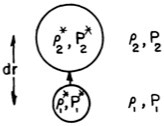
\includegraphics[width=(0.3\textwidth),height=(\textheight-11mm),keepaspectratio]{conv_stab}
\caption{Perturbation of radiative layer to test for stability against convection.}
\end{figure}

After the perturbation the density may differs now from that of the surroundings since internal density is determined by adiabatic transformation of the element
\begin{align*}
P_2=P_2^*,\quad\rho_2^*=\rho_1^*(\frac{P_2^*}{P_1^*})^{\frac{1}{\gamma}}&\intertext{where $\gamma=\frac{c_P}{c_v}$ is the ratio of specific heat and has the value $\frac{5}{3}$ for highly ionized gas}
\end{align*}

The pressure force exerted on that volume which the element occupies after its displacement and expansion has not be alterated by the perturbation, the gravitational force will be altered if the density within the element after the perturbation differs from that in the surroundings.

Condizione di stabilit\'a
\begin{align*}
\rho_2^*>\rho_2&\intertext{I can trasform this condition in a more practical one: sobstituting expression for the variables of surroundings and taking taylor's expansion of the quantities at higher position:}\\
-\frac{1}{\gamma}\frac{1}{P}\TDy{r}{P}<-\frac{1}{\rho}\TDy{r}{\rho}
\end{align*}

For the cases where the equation of state for an ideal gas hold I can take logarithimic derivative of $P=\frac{k}{\mu}\rho T$ and thus I can express density gradient in terms of temperature and pressure gradient:

\begin{align*}
-(1-\frac{1}{\gamma})\frac{T}{P}\underbrace{\TDy{r}{P}}_{\text{from HE}}>-\underbrace{\TDy{r}{T}}_{\text{from RE}}&\intertext{since both temperature gradient and pressure gradient are negative both sides of $\uparrow$ are positive. Right side contains absolute value of temperature gradient, left side contains the adiabatic temperature gradient (would represent temperature gradient if the temperature and pressure followed the adiabatic relationship through the layer).}
\end{align*}

For a layer to be stable against convection the actual temperature gradient must be lower in absolute value than the adiabatic temperature gradient.\index{Stability condiction against convection: Schwarzschild.}

The above condiction hold only in homogenous layers.


\section{Meccanismi che contribuiscono  all'opacit\'a.}

\subsection{Radiation and equilibrium}

\begin{definition}{Emission coefficient.}
\begin{align*}
&j_{\nu}=m\,d\omega\,dt\,d\nu&\intu{amount of radiant energy emitted: $j_{\nu}$ is the emission coefficient for frequency $\nu$.}
\end{align*}
\end{definition}

\begin{definition}{Einstein coefficients.}
\begin{itemize}
\item Spontaneous emission.

The probability that in a interval of time $dt$ an atom in an excited state n emits a quantum of energy $h\nu_{mn}$ in the solid angle $d\omega$ in absebce of external field is $A_{nm}\,d\omega\,dt$: this spontaneous emission take place uniformly in all direction.

\item Stimulated emission.

The probability that an excited atom in state n is stimulated by external field of radiation to emit a quantum $h\nu_{nm}$, in the direction $d\omega$, in time $dt$ is given by $B_{nm}I_{\nu_{nm}}\,d\omega\,dt$, where $I_{\nu_{nm}}$ is the intensity of radiation of frequency $\nu_{nm}$ at the point where the atom is located and in the direction $d\omega$: the induced emission of radiation by a given pencil of radiation take place in the same direction as incident pencil.

\end{itemize}

In condizioni di equilibrio termodinamico
\begin{equation*}
j_{\nu}=\kappa_{\nu}B_{\nu}(T)
\end{equation*}
where T is the (local) temperature.

If there are $N_m$ atoms in n-th state per unit volume
\begin{align*}
&\frac{A_{nm}}{B_{nm}}=\frac{2h\nu_{nm}^3}{c^2}\\
&\frac{N_mB_{mn}}{N_nB_{nm}}=\exp{\frac{h\nu_{nm}}{KT}}
\end{align*}

\end{definition}

Vedi Chandrasekhar pg 190

\subsection{Electron scattering.}

Lo scattering da parte di un elettrone di un'onda EM incidente ovvero, l'emissione di dipolo di un'elettrone oscillante indotta da un'onda elettromagnetica \'e equivalente all'assorbimento del fotone:
\begin{align*}
&\sigma_e=\frac{8\pi}{3}(\frac{e^2}{m_ec^2})^2=\SI{6.652e-25}{\square\cm}&\intu{Thomson cross-section, the associated opacity coefficient is due to combined effect of all electrons in a unit mass of gas}\\
&\kappa_{es}=\frac{\sigma_e}{\frac{\rho}{n_e}}=\frac{\sigma_e}{\mu_em_u}&\intertext{for totally ionized gas $\mu_e=\frac{2}{1+X}$:}\\
&\kappa_{es}=0.20(1+X)\si{\square\cm\per\gram}
\end{align*}

Electon scattering is important source of opacity in ionized gas not too dense. When degree of ionization drops ($T\leq\SI{e4}{\kelvin}$, in H-rich gas) the electron density become so small that  $\kappa_{es}$ is strongly reduced.

\subsubsection{Energetic photons: Effetto Compton.}

When photon energy becomes significant fraction of rest mass of electron $h\nu\geq0.1m_ec^2$ the exchange of momentum between photon and electron must be taken in account (Compton scattering): at high temperature since maximum of Plank function is at \mblock{h\nu=4.965 KT,\ KT\geq0.02m_ec^2} or $T\geq\SI{e8}{\kelvin}$: At high temperature the electron scattering opacity is reduced.

\subsection{Free-free absorption.}

A free electron cannot absorbs a photon because of momentum/energy conservation; it can happens if there is an EM with a close ion: it's the inverse process of bremsstrahlung. The derivation of absorption coefficient is a QM problem: an approximate calculation is the Kramer's law.

\subsubsection{Kramer's law.}

The absorption efficiency of the temporary electron-ion system is proportional to $Z_i^2\nu^{-3}$

\begin{align*}
&\kappa_{\nu}^{ff}\propto\frac{n_e}{\rho}\sum_in_iZ_i^2T\expy{-\frac{1}{2}}\nu^{-3}&\intu{cross-section of ion i:}\\
&\overline{v}=\sqrt{\frac{3KT}{m_e}}\\
&\Delta t\propto1/\overline{v}\propto T\expy{-\frac{1}{2}}&\intu{time of effective ion-electron coupling.}\\
&\sigma^{ff}_i\propto n_eT\expy{-\frac{1}{2}}Z_i^2\nu\expy{-3}&\intertext{the opacity coefficient follows by multiplying $\uparrow$ by $\frac{n_i}{\rho}$.}\\
\end{align*}

In a completely ionized gas $\frac{n_e}{\rho}=\frac{1}{\mu_em_u}=\frac{1+X}{2m_u}$.

\begin{align*}
&\kappa_{ff}\propto\rho T\expy{-\frac{7}{2}}\\
&\kappa_{ff}\propto\num{3.8e22}\rho T\expy{-\frac{7}{2}}\si{\square\cm\per\gram}
\end{align*}

We have to the into account of QM effects with the Gaunt factor.

\subsection{Bound-free, bound-bound absorption.}

\begin{itemize}
\item Bound-free absorption is the absorption of a photon by a bounded electron where the photon energy exceed ionization energy $\chi$. Classical consideration lead to formula of the Kramer form.
\item Bound-Bound absorption. Efficient because the absorption lines are broadened by collisions. Important for $T\leq\SI{e6}{\kelvin}$.
\item Bound-free absorption of negative hydrogen ion ($\chi=\SI{0.75}{\ev}$). Important in cool stars or solar atmosphere. The resulting opacity is sensitive to metallicity and temperature: the free electrons to make ion come from single ionized metals such as Na, K, Ca, Al.
\item Dust and molecules. In cool stars with $\teff\leq\SI{4000}{\kelvin}$ opacity from molecules and dust grain ($T\leq\SI{1500}{\kelvin}$) becomes dominant.
\end{itemize} 

\subsubsection{Negative H ion}

\subsection{Temperature-density diagram for the opacity.}

\begin{todo}{Temperature-density diagram for the opacity}
Schwarzschild pg 67-73
\end{todo}

\begin{figure}[!ht]
\centering
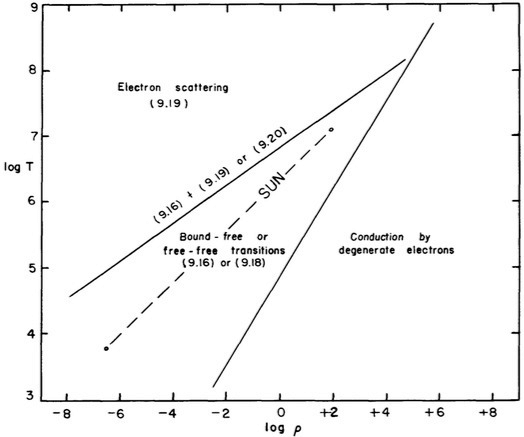
\includegraphics[width=(0.9\textwidth),height=(\textheight-11mm),keepaspectratio]{kappaqu}
\caption{Temperature-density diagram for the opacity.}
\end{figure}

\clearpage

\section{Relazione Massa-Luminosit\'a}

\subsection{Stability of thermal equilibrium}

Estimate of luminosity in the sun midway between center and surface.

\begin{align*}
&L_r=4\pi r^2\frac{4ac}{3}\frac{T^3}{\kappa\rho}\TDy{r}{T}&\intertext{$\uparrow$ radiative equilibrum plus crude estimates:}\\
&\kappa\rho\approx1cm,\quad T\approx10\sci{6}\,K&\intertext{taking for differnetial the difference I have:}\\
&L\approx6\sci{35}&\intertext{$\uparrow$ exceeds the luminosity of the sun by a factor 100.}
\end{align*}

How does the luminosity of a star depends on its mass?

\begin{align*}
&L_r=4\pi r^2\frac{4ac}{3}\frac{T^3}{\kappa\rho}\TDy{r}{T}&\intertext{$\uparrow$ radiative equilibrum plus crude estimates:}\\
&\rho\propto \frac{M}{R^3}&\intertext{introducing this proportionality in hydrostatic equilibrium equation $\downarrow$}\\
&\TDy{r}{P}=-\frac{Gm(r)\rho}{r^2}&\intertext{we find the dependence of representative pressure on the mass and radius $\downarrow$}\\
&P\propto\frac{M^2}{R^4}&\intertext{from equation of state for ideal gas, $T\propto\frac{P}{\rho}$, we have $\downarrow$}\\
&T\propto\frac{M}{R}&\intertext{introducing the proportinalities for T and P in radiative equilibrium equation we obtain:}\\
L\propto M^3
\end{align*}

\index{Mass-Luminosity relation: radiative equilibrium condition.}

The above estimates point out that the luminosity of a star is not determined by the rate of energy generation by nuclear process: only radiative equilibrium condition enters in the derivation.

The pressure force must counteract gravity according to HE equation: if the pressure have to be high enough for this porpuse the internal temperature must have certain relatively high values according to equation of state. The temperature gradient from hot internal zone to cold surface will cause a net radiation flux according to 
\begin{equation*}
l(r)=-4\pi r^2\frac{4ac}{3}\frac{T^3}{\kappa\rho}\TDy{r}{T}
\end{equation*}

The stength of this radiation flux will be fixed by radiative equilibrium condition irrespective of whether or not the the energy loss is compensate by nuclear energy production in the interior. If the energy loss by radiation at the surface is bigger the nuclear energy generation the suffers a net energy loss: this can made up from gravitational energy by contraction. During the contraction one half of the gravitational energy is available for radiation losses from surface, the other half go into increase of thermal energy. The contraction will stops when the over-all rate nuclear energy release is equal to radiative surface losses.


\subsection{Relazione massa luminosit\'a: limite di Eddington.}

Ipotesi:
\begin{itemize*}
\item Trasporto in superficie \'e radiativo conduttivo
\item $\kappa$ \'e approx costante
\item La pressione di radiazione fornisce un contributo dominante alla pressione totale
\end{itemize*}

Se la pressione di radiazione fornisce un contributo dominante $P\approx P_r$ ho
\begin{align*}
&\TDy{r}{P_r}=-\frac{\kappa_{\nu}}{c}\rho\frac{l(r)}{4\pi r^2}&\intertext{$\uparrow$ LTE}\\
&\PDy{r}{P}\approx\PDy{r}{P_r}=-\frac{Gm(r)\rho}{r^2}&\intertext{$\uparrow$ equilibrio idrodinamico}\\
&L=l(R)=GM\frac{4\pi c}{\kappa}&\intertext{Stimo il valore della costante di proporzionalit\'a fra massa e luminosit\'a nel caso di stelle massicce $\beta=\frac{P_g}{P}\approx0$:}\\
&\frac{L}{\lsun}\approx\sci{4}\frac{M}{\msun}&\intertext{$\uparrow$ \'e un limite superiore: limite di Eddington. Utile per studio dei nuclei galatticci. Utilizzando il modello di Eddington ($\beta=const$) invece ho:}\\
&\TDy{r}{P_r}=(1-\beta)\TDy{r}{P}=-(1-\beta)\frac{Gm(r)}{r^2}\rho&\intertext{quindi}\\
&L\approx[1-\beta(M)]\sci{4}(\frac{M}{\msun})\lsun&\intertext{Per piccole masse $\beta\approx1$ e quindi $1-\beta(M)\propto M^2$ ho:}\\
&L\propto M^3
\end{align*}

\subsection{Tempo di vita per oggetti che si avvicinano al limite di Eddington}

Energia disponibile
\begin{align*}
E_d=\alpha Mc^2&\intertext{$\alpha\approx0.01$ per reazioni nucleari, $\alpha\approx1$ per oggetti massicci.}
\end{align*}

Stimo il tempo di vita sulla base dell'energia disponibile
\begin{align*}
&T_{Max}=\frac{E_d}{L}\approx\frac{\alpha Mc^2}{\sci{4}M\lsun/\msun}=\alpha T_0\\
&=\alpha*(2\sci{9}\,yr)
\end{align*}


\section{Conductive transport of energy}

\subsection{Conduction in ordinary stellar matter}

In ordinary stellar matter conduction has no chance of taking over an appreciable part of the total energy transport.

Although the small collisional cross section for particles of ionized gas the large density result in a $l_{gas}$ several orders of magnitude smaller than $l_{ph}$ and velocities are few percent of c.

\subsection{Conduction in degenerate stellar interior}

In the core of evolved stars where the electron gas is highly degenerate conduction becomes efficient. Gli elettroni sono pi\'u vicini all'energia di Fermi e poich\'e le celle dello spazio delle fasi sono piene le collisioni in seguito a cui cambia il momento sono improbabili: il coefficiente di diffusione aumenta.

\subsection{Heat transfer equation}

\begin{align*}
&\PDy{m}{l}=\epsilon-\PDy{t}{u}+\frac{P}{\rho^2}\PDy{t}{\rho}&\intertext{$\uparrow$ equation of local energy equilibrium. Sostituisco in $\uparrow$ le espressioni $\downarrow$:}\\
&l=-\sigma^*\PDy{m}{T},\quad u=c_vT&\intertext{quindi}\\
&\PDof{m}(\sigma^*\PDy{m}{T})-c_v\PDy{t}{T}=-[\epsilon+\frac{P}{\rho^2}\PDy{t}{\rho}]&\intertext{se pongo il lato destro uguale a zero ho un'equazione che ha la forma dell'equazione di trasporto di calore con conducibilit\'a $\sigma^*$. nel caso di un problema unidimensionale ho}\\
&\PDof{x}(\sigma\PDy{x}{T})=c\PDy{t}{T}&\intertext{La soluzione di $\uparrow$ con le condizioni al bordo tende alla soluzione costante dopo un tempo sufficiente:}\\
&T(x,t)\to T(x)=const
\end{align*}

Timescale of thermal adjustment.

\begin{align*}
&\tau_{Adj}=\frac{c}{\sigma}d^2&\intertext{Eqution of heat transfer demand the characterisc time $\uparrow$ with d is a characteristic lenght over which the initially given $T(x)$ function changes. For a star (\mblock{\PDof{m}\to\frac{1}{M}}, \mblock{L\approx\frac{\sigma^*\overline{T}}{M}}):}\\
&\tau_{Adj}=\frac{c_vM^2}{\overline{\sigma^*}}\ \Rightarrow \ L=\frac{E_i}{T}=\frac{\overline{\sigma}^*\overline{T}}{M}
\end{align*}

Nel caso di stelle degeneri
\begin{align*}
&\tau_{Adj}\approx\frac{c_v\overline{T}M}{L}=\frac{E_i}{L}=\tkh&\intertext{$\uparrow$ when energy is efficiently transported by conduction.}
\end{align*}


\section{Radiative equilibrium. Eddington luminosity.}

\subsection{Radiation pressure gradient}

Il trasporto radiativo implica un gradiente di temperatura non nullo e quindi un gradiente della pressione di radiazione dato da

\begin{align*}
&\TDof{r}(P_{Rad})=\TDof{r}(\frac{1}{3}aT^4)=\frac{4}{3}aT^3\TDy{r}{T}\\
&=-\frac{\kappa\rho}{4\pi c}\frac{l}{r^2}&\intertext{Radiation pressure gradient represents an outward force due to net flux of photons.}
\end{align*}

\subsection{Upper limit to local luminosity}

For a star in hydrostatic equilibrium the outward radiation force must be smaller than the inward force of gravity as given by pressure gradient necessary for HE

\begin{align*}
&|\TDy{r}{P_{Rad}}|<|(\TDy{r}{P})_{HE}|\quad\Rightarrow\quad\frac{\kappa\rho}{4\pi c}\frac{l}{r^2}<\frac{Gm\rho}{r^2}\\
&l<\frac{4\pi cGm}{\kappa}=l_{Edd}\index{Luminosit\'a di Eddington}&\intertext{$\uparrow$ is the max luminosity that can be carried by radiation inside a star in HE}\\
\end{align*}

\subsection{Convective energy transport}

The Eddington limit for local luminosity of a star can be violated in case of very large flux (as for intense nuclear burning) or in case of very high opacity (outer layers of the sun: rel. low T near the ionization temperature of H and He). In such cases hydrostatic equilibrium and radiative equilibrium can't hold together, therefore if the star is to remains in HE energy must be transported by different mean than radiative diffusion: convection, the collective motion of gas bubbles that carry heat and can distributes it efficiently.

\subsection{Necessary condition for stability against convection}

\begin{align*}
&L<L_{Edd}=\frac{4\pi GM}{\kappa}&\intertext{For the surface of a star:}\\
&L_{Edd}=3.8\sci{4}(\frac{M}{\msun})(\frac{0.34cm^2/g}{\kappa})\lsun&\intertext{$\uparrow$: $\kappa$ is the opacity of photosphere, $0.34cm^2/g$ correspond to electron scattering opacity for $X=0.7$.}
\end{align*}


\subsection{Stability condition for radiative equilibrium: relation between convection criterion and Eddington limit.}

If we want construct a stable model of a star every layers of the star must have such properties that every small fluctuation is smeared away. That is pressure gradient must be computed from hydrostatic equilibrium condition $\TDy{r}{P}=-g(r)\rho=-\rho G\frac{m(r)}{r^2}$, the temperature gradient from the radiative equilibrium condition $l(r)=-4\pi r^2\frac{4ac}{3}\frac{T^3}{\kappa\rho}\TDy{r}{T}$ and both gradients have to be inserted in the condition dynamical stability

\begin{equation*}
-(1-\frac{1}{\gad})\frac{T}{P}\TDy{r}{P}>-\TDy{r}{T}
\end{equation*}

To relate the convection criterion for stability, $\nrad{}<\nad{}$ (\sch{} criterion) with $\nrad{}=(\TDly{P}{T})_{Rad}=\frac{3}{16\pi acG}\frac{\kappa lP}{mT^4}$ temperature gradient if the entire energy flux is transported by radiation, to the Eddington limit we write $\nrad{}$ in terms of $l$ and $l_{Edd}=\frac{4\pi cGm}{\kappa}$ and $P_{Rad}=(1-\beta)P$:

\begin{align*}
l<4(1-\beta)\nad{}l_{Edd}&\intertext{$\uparrow$ \sch{} criterion in terms of $l$ and $l_{Edd}$. For $\beta>0$ and $\nad{}>0.25$ convection sets in before Eddington limit is reached.}
\end{align*}


\section{$(L,M,R)$ relations.}

\subsection{Maximum mass for main sequence stars. }

In very luminous main-sequence stars the opacity is dominated by electron scattering. I can assume $\kappa$ constant.

\begin{align*}
L_{Edd}\propto M&\intertext{while for stars (at least in the main sequence: $x\approx3.5$)}\\
L\propto M^x,\quad x>1&\intertext{We can expect a maximum mass for main-sequence stars.}
\end{align*}

\index{Mass-luminosity relationship: limite superiore per sequenza principale}


\subsection{Rough estimate of Mass-Luminosity relationship.}

Estimate of luminosity in the sun midway between center and surface.

\begin{align*}
&L_r=4\pi r^2\frac{4ac}{3}\frac{T^3}{\kappa\rho}\TDy{r}{T}&\intertext{$\uparrow$ radiative equilibrum plus crude estimates:}\\
&\kappa\rho\approx1cm,\quad T\approx10\sci{6}\,K&\intertext{taking for differnetial the difference I have:}\\
&L\approx\num{6e35}&\intertext{$\uparrow$ exceeds the luminosity of the sun by a factor 100.}
\end{align*}

How does the luminosity of a star depends on its mass?

\begin{align*}
&L_r=4\pi r^2\frac{4ac}{3}\frac{T^3}{\kappa\rho}\TDy{r}{T}&\intertext{$\uparrow$ radiative equilibrum plus crude estimates:}\\
&\rho\propto \frac{M}{R^3}&\intertext{introducing this proportionality in hydrostatic equilibrium equation $\downarrow$}\\
&\TDy{r}{P}=-\frac{Gm(r)\rho}{r^2}&\intertext{we find the dependence of representative pressure on the mass and radius $\downarrow$}\\
&P\propto\frac{M^2}{R^4}&\intertext{from equation of state for ideal gas, $T\propto\frac{P}{\rho}$, we have $\downarrow$}\\
&T\propto\frac{M}{R}&\intertext{introducing the proportinalities for T and P in radiative equilibrium equation we obtain:}\\
L\propto M^3
\end{align*}

\index{Mass-luminosity relationship (Rough)}

\subsection{LL e C}


\chapter{Dynamical instability. Convective energy transport.}
\PartialToc

\section{Dynamical instability}

\subsection{Small fluctuation in concentric shell}

Until now we have supposed perfect spherical symmetry: all function and variables are constant on a concentric sphere. In reality will arise small fluctuations on such a sphere: these local perturbation may be ignored if it don't grow.

In the basic equations spherical symmetry can be kept if we interpret the variables as a proper average over a concentric sphere. 

\subsection{Local description for the stability of a layer: mass elements and average surroundings.}

In local description we represent a fluctuation by mass element $(e)$ in which the functions have constant but somewhat different values then in the average surroundings

\begin{figure}[!ht]
\centering
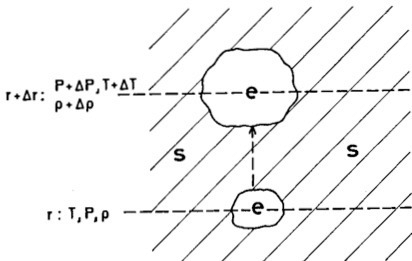
\includegraphics[width=(0.6\textwidth),height=(\textheight-11mm),keepaspectratio]{esconv}
\caption{Test of stability of a layer.}
\end{figure}

We suppose that the moving elements have no time to exchange appreciable amlount of heat with the surroundings: adiabatic movement (Dynamical instability).

Difference between the element and surroundings
\begin{equation*}
DA=A_e-A_s
\end{equation*}

\begin{itemize*}
\item For $DP\neq0$ expansion/contraction occurs at sound speed: much more rapid than other motions of elements.

We can suppose $DP=0$.

\item Let's suppose an initial fluctuation in T, $DT>0$: $DT>0$ requires that, for ideal gas ($\rho\propto\frac{P}{T}$), $D\rho<0$: the element is lighter than surroundings material, temperature fluctuations are accompained by radial local motion.

\item Let's suppose a radial displacement $\Delta r$
\begin{align*}
&D\rho=[(\TDy{r}{\rho})_e-(\TDy{r}{\rho})_s]\Delta r&\intertext{the terms in squares are change in density of the element while rises $dr$ minus spatial gradient of the surroundings}
\end{align*}

A finite $D\rho$ gives the radial component \mblock{K_r=-gD\rho} of a buoyancy force per unit of mass (g is the gravity acceleration): if $D\rho<0$ the perturbation is increased by the $K_r>0$

\end{itemize*}

Convection instability leads to cyclic macroscopic motion but the star is still in overall hydrostatic equilibrium.

\section{Condition for stability for radial fluctiations.}

\subsection{Condition for stability: density gradient}

For a radial upward fluctiation of an element:

if $D\rho<0$ the element is lighter and $K_r>0$, the situation is unstable.

If $D\rho>0$ the $K_r<0$: the element is drawn back to its original position: the layer is stable.

\begin{align*}
&(\TDy{r}{\rho})_e-(\TDy{r}{\rho})_s>0&\intertext{$\uparrow$ is highly impractical}
\end{align*}

\subsection{Condition for stability: temperature's and mean molecular weight's gradient}

\begin{align*}
&\frac{d\rho}{\rho}=\alpha\frac{dP}{P}-\delta\frac{dT}{T}+\phi\frac{D\mu}{\mu}&\intertext{with the coefficients:}\\
&\alpha=\Dcvar{\PDly{P}{\rho}}{T,\mu},\   \delta=\Dcvar{\PDly{T}{\rho}}{P,\mu},\\ &\phi=\Dcvar{\PDly{\mu}{\rho}}{T,P}&\intertext{For ideal gas:}\\
&\rho\propto\frac{P\mu}{T},\quad \alpha=\delta=\phi=1, d\mu_e=0\\
&-(\frac{\delta}{T}\TDy{r}{T})_e+(\frac{\delta}{T}\TDy{r}{T})_s-(\frac{\phi}{\mu}\PDy{r}{\mu})_s>0&\intertext{}
\end{align*}

\subsection{Scale height of pressure}

\begin{align*}
&H_P=-\frac{dr}{d\,\ln{P}}=-P\frac{P}{r}\\
&H_P=\frac{P}{\rho g}, \quad \PDy{r}{P}=-g\rho&\intertext{$H_P$ has the dimension of a length and its value represents the characteristic scale of radial pressure variation.}\\
&\parbox{1.3cm}{Solar photosphere:}\left\{\begin{array}{c}
g=2.7 \sci{4}\,cm\,s^{-2} \\
P=6.8\cdot\sci{4}\,dyn\,cm^{-2}\\
\rho=1.8\sci{-7}\,g\,cm^{-3}\\
\end{array}\right.\\
&\Rightarrow H_P=1.4\sci{7}\,cm\\
&r=\frac{\rsun}{2}:\ \left\{\begin{array}{c}
g=1.0 \sci{5}\,cm\,s^{-2} \\
P=6.7\cdot\sci{14}\,dyn\,cm^{-2}\\
\rho=1.3\,g\,cm^{-3}\\
\end{array}\right.\\
&\Rightarrow H_P=5.2\sci{9}\,cm
\end{align*}

\subsection{Condition for stability: adiabatic Temperature gradient (\sch{}).}

Anticipo il criterio di \sch{} di \ref{ssec:schcstab}.

Abbiamo visto che piccole fluttuazioni radiali di quantit\'a di materia di uno strato sferico di una stella (per esempio spostamento vero l'alto) avvengono in equilibrio di pressione con gli strati attraversati dalla porzione di materia:

The expansion of the gas element as it rises $\Delta r$ occurs on the local dynamical timescale (with  the speed of sound) and therefore the displacement and expansion of the gas element will be very close to adiabatic.

\begin{align*}
\frac{\delta P_e}{P_e}=\gamma_{Ad}\frac{\delta \rho_e}{\rho_e}&\intertext{$\gamma_{Ad}$ is the adiabatic exponent:}\\
\gamma_{Ad}=(\TDly{\rho}{P})_{Ad}\\
\TDly{P}{\rho}>\frac{1}{\gamma_{Ad}}&\intertext{$\uparrow$ criterion for stability against convection: the density gradient must be steeper than a critical value determined by $\gamma_{Ad}$}
\end{align*}

\begin{figure}[!ht]
\centering
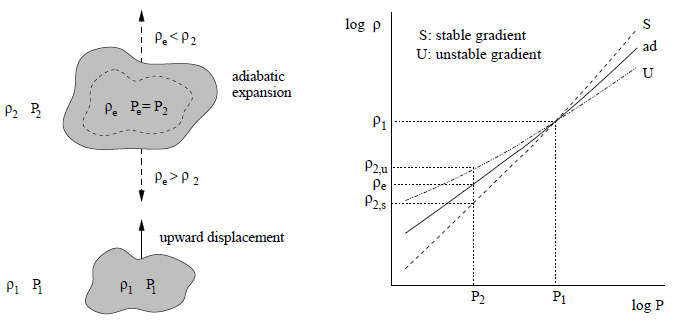
\includegraphics[width=(\textwidth),height=(\textheight-11mm),keepaspectratio]{acvsadTgrad}
\caption{A layer is stable against convection if the density varies more steeply with pressure than for an adiabatic change.}
\end{figure}

\clearpage

\section{Condiction for stability against convection: Ledoux, Schwarzschild criteria}

The following criteria to test the stability of layers against convection are local ones: easily evaluated at given place given local $P$, $T$, $\rho$ only.
\index{Local criteria for convection stability}
In extreme cases the local forces must be coupled to the neighbouring layers by momentum transfer, inertia continuity equation.

\subsection{General condition for stability: use of pressure scale height}

\begin{align*}
H_P[-(\frac{\delta}{T}\TDy{r}{T})_e+(\frac{\delta}{T}\TDy{r}{T})_s-(\frac{\phi}{\mu}\TDy{r}{\mu})_s]>0
\end{align*}

\subsection{Ledoux's criterion}

Riscrivo il criterio di stabilit\'a per fluttuazioni radiali in forma simbolica

\begin{align*}
&\underbrace{(\TDly{P}{T})_s}_{\nabla}<\underbrace{(\TDly{P}{T})_e}_{\nabla_e}+\frac{\phi}{\delta}\underbrace{(\TDly{P}{\mu})_s}_{\nabla_{\mu}}&\intertext{$()_s$ are both spatial derivatives in which P is taken as a measure of depth, $\nabla_e$ is the variation of T in the element during the motion (position is measured by P).}\\
&\nablaTact<\nel+\frac{\phi}{\delta}\nmu
\end{align*}

In a layer that transport all energy by radiation $\nablaTact=\nrad$, let's test such a layer for stability. We have supposed adiabatic change for the element fluctuations $\nel=\nad$.
We have the Ledoux criterion for stability of a radiative layer against convection (dynamical stability)

\begin{align*}
\nrad<\nad+\frac{\phi}{\delta}\nmu
\end{align*}

$\nmu\neq0$ in interior of evolving stars where heavier elements are usually produced below the lighter ones: molecular weight increases inward and the relative terms in the stability condition has a stabilizing effect ($\delta$, $\phi$ are positive).

\subsection{Schwarzschild's criterion}\label{ssec:schcstab}

In regions with homegenous chemical composition $\nmu=0$.
We have the Schwarzschild criterion for the stability of a radiative layer

\begin{align*}
\nrad<\nad
\end{align*}

\subsection{Causes of instability}

According to Schwarzschild criterion convection occurs when $\nrad=\frac{3}{16\pi acG}\frac{P}{T^4}\frac{\kappa l}{m}>\nad$.

Zones where we may found convective instability
\begin{itemize*}

\item Opaque region of stars: large value of $\kappa$. For example in outer regions of the Sun because opacity increses with decreasing temperature. Since low mass stars are cooler than high mass stars we may expect the former to have convective envelopes.

\item Regions with a large value of $\frac{l}{m}$ are regions with large energy flux. Toward the center of a star $\frac{l}{m}\approx\epsilon_{nuc}$: stars with nuclear energy production strongly peaked toward the center can be expected to have a convective core. That is the case of massive stars. 

\item We can have small values of $\nad$ in the zones of partial ionization of H and He at relatively low temperature and, even if the opacity is small the surface layers of stars may be unstable against convection. Stars of all masses have  shallow surface  convection zones at temperatures where lighter elements are partially ionized.

\end{itemize*}

\subsection{Convective zones in $\msun$ and $4\msun$ stellar model.}

\begin{figure}[!ht]
\centering
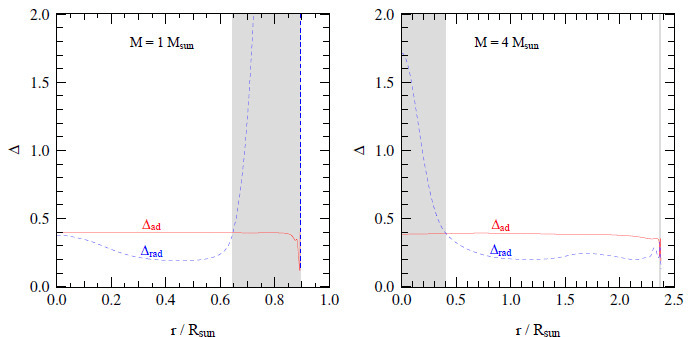
\includegraphics[width=(0.9\linewidth),keepaspectratio]{shallowconv}
\caption{Variation of $\nad$ and $\nrad$ with radius in two models at the start of main sequence.}
\end{figure}

In both models $\nad\approx0.4$ since conditions are close to an ideal gas, in the surface ionization zones $\nad<0.4$ and a thin convective layer appears in the $4\msun$ model.

The solar mass model has a very large opacity in its outer layer, resulting in a large value of $\nrad$ which gives rise to convective envelope where $\nrad>\nad$ (gray shading).

The $4\msun$ model has a hotter outer envelope with lower opacity so that $\nrad$ stay small; the large energy generation rate in the center result in a convective core.

\clearpage

\subsection{Sketch of temperature gradients}

For an unstable layer violating the \sch{} criterion we can plot the different gradients: in a $\ln{P}-\ln{T}$ diagram an adiabatic change follows a line with slope $\nad{}$, the changes in a rising element are given by $\nel{}$, while the stratifications in the surroundings and in a radiative layer are shown by lines with slopes $\nablaTact{}$ and $\nrad{}$ respectively.

Suppose $\nmu{}=0$ it follows from the violation of genaral condition for dynamic stability in the general case

\begin{equation*}
\nablaTact<\nel+\frac{\phi}{\delta}\nmu
\end{equation*}
that is $\nablaTact{}>\nel{}$. If some part of the flux is carried by convection then $\nablaTact{}<\nrad{}$ (that is to say if the entiere energy flux would be transported by radiation the actual T gradient would be greater).

Let's consider a rising element starting from $(P_0,T_0)$: this element moves downward to the left corner along the line with slope  $\nel{}$. Since $\nablaTact{}>\nel{}$, the element, although cooling, will have an increasing temperature excess over its new surroundings: it will radiates energy into its surroundings which means that the element cools more than adiabatically: $\nel{}>\nad{}$.\index{"Super-adiabatic" cooling}

\begin{align*}
\nrad{}>\nablaTact{}>\nel{}>\nad{}&\intertext{The fact that element's temperature gradient must always be between adiabatic and surroundings temperature gradients shows that the Ledoux and \sch{} criteria are also to be used in near-surface regions where the rising elements lose much of their energy by radiation:}\\
\nrad{}<\nel{}<\nad{}&\intertext{$\uparrow$ for a convective stable layer where $\nel{}>\nad{}$.}
\end{align*}

\begin{figure}[!ht]
\centering
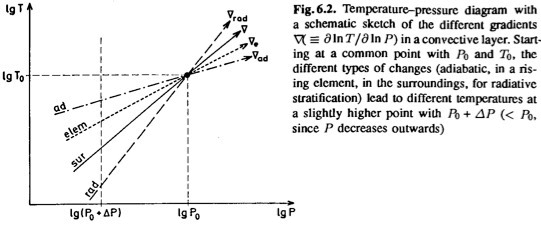
\includegraphics[width=(\textwidth),height=(\textheight-11mm),keepaspectratio]{Tgrads}
\caption{Temperature-pressure diagram with a schematic sketch of the different gradients in convective unstable layer.}
\end{figure}

\clearpage


\section{Oscillation of displaced elements}

\subsection{Equation of motion for mass elements in dynamically stable layers}

In a dynamically stable layer mass elements can oscillate around the equilibrium position because of fluctuations. Consider $\Delta r>0$

\begin{align*}
&D\rho=\frac{\rho\delta}{H_P}[\nel{}-\nablaTact{+\frac{\phi}{\delta}}\nmu{}]\Delta r&\intertext{$\uparrow$ excess of density. Remembering:}\\
&\delta=-(\PDly{T}{\rho}),\ \phi=-(\PDly{\mu}{\rho}),\\ &H_P=-\frac{dr}{d\ln{P}}=-P\TDy{P}{r}\\
&\nablaTact{}=\nablaTacte{},\ \nel{}=\nele{},\\
&\nmu{}=\nmue{}
\end{align*}

In presence of gravity acceleration g the buoyancy force per unit volume is
\begin{align*}
&K_r=-gD\rho&\intertext{producing an acceleration of the element}\\
&\PtwoDy{t}{\Delta r}=-\frac{g\delta}{H_P}[\nel{}-\nablaTact{}+\frac{\phi}{\delta}\nmu{}]\Delta r&\intertext{the righthand side is negative since in a stable layer $\frac{D\rho}{\Delta r}>0$ and thge solution of the equation of motion is of the form}\\
&\Delta r=\Delta r_0\exp{i\omega t}&\intertext{$\uparrow$ oscillations around equilibrium position.}
\end{align*}

\subsection{Frequency of oscillations: the Brunt-V\"ais\"al\"a frequency.}

The frequency of this adiabatic oscillation is the Brunt-\vai{} frequency
\begin{align*}
&\omega^2_{Ad}=\frac{g\delta}{H_P}(\nad{}-\nablaTact{}+\frac{\phi}{\delta}\nmu{})&\intertext{in unstable layers $\omega^2<0$.}
\end{align*}

\subsection{Radiative correction.}\label{ssec:radlosscil}

Suppose $DT>0$, superpose to radial energy flux $\vec{F}$, carrying energy from stellar interior to the surface, there will be a local non-radial flux $\vec{f}$, carrying the surplus energy of the element to its surroundings: the radiative flux from the elements due to its temperature excess will be

\begin{align*}
&f=\frac{4acT^3}{3\kappa\rho}|\PDy{n}{T}|&\intertext{$\PDof{n}$ is differenziation perpendicular to the surface of the element:}\\
&\PDy{n}{T}\approx\frac{2DT}{d}\\
&\lambda=Sf=\frac{8acT^3}{3\kappa\rho}DT\frac{S}{d}&\intertext{$\uparrow$ radiative loss per unit of time from the surface S of the blob, it determines the rate by which the thermal energy of the blob of volume V changes:}\\
&-\lambda=\rho Vc_P\PDy{t}{T_e}\approx\rho Vc_P\PDy{t}{DT}\\
&\PDof{t}(DT)=-\frac{DT}{\tau_{Adj}}&\intertext{$\uparrow$ ho introdotto il tempo caratteristico $\tau_{Adj}$ che \'e approx l'eccesso di calore diviso la luminosit\'a:}\\
&\tau_{Adj}=\frac{\rho Vc_P DT}{\lambda}=\frac{\kappa\rho^2c_Pd^2}{16acT^3}&\intertext{for large elements far from regions of marginal stability:}\\
&\tau_{Adj}\gg\frac{1}{\omega_{Ad}}
\end{align*}

Radiative loss gives a small deviation from adiabatic oscillations.

\section{Mixing length theory}

\subsection{Convective equilibrium}

Let's consider a layer in which the stability condition ($\downarrow$) is not fulfilled
\begin{align*}
&-\frac{1}{\gamma}\frac{1}{P}\TDy{r}{P}<-\frac{1}{\rho}\TDy{r}{\rho}\\
&-(1-\frac{1}{\gamma})\frac{T}{P}\TDy{r}{P}>-\TDy{r}{T}
\end{align*}

Hence upon the slightest perturbation convective motions will break out throughout the unstable layer: a perturbed element which is displaced upwards will have an internal density lower than the surrounding density, it experiences a net upwards force and will continues its upward motion. Similarly for an element displaced downwards.
Both downward and upward moving elements contribute to a convective energy transport upwards.

Assume initially that the layer is in precarious radiative equilibrium with the radiative flux carrying out the energy produced by nuclear processes.

Now because of instability convective motion break out throughout the layer: convective motions will transport thermal energy from lower levels to upper levels of the layer. Thus the temperature gradient will be reduced by convection and thus will be reduced the radiation flux according to equation for radiative equilibrium and the thus will be reduced also the convective energy flux since a reduction of the excess of the actual temperature gradient over the adiabatic temperature gradient.

The lowering of temperature gradient by convection will continue until the radiation flux and convective flux together fulfill the basic thermal equilibrium condition
\begin{equation*}
\TDy{r}{l(r)}=\epsilon\rho4\pi r^2
\end{equation*}

Thus instability of radiative equilibrium of a layer of a star leads to the state of convective equilibrium.

\subsection{Local flux of energy}

In an unstable layer the total flux is 

\begin{align*}
&F_{Rad}+F_{Con}=\frac{l}{4\pi r^2}=\frac{4acG}{3}\frac{T^4m}{\kappa Pr^2}\nrad{}\\
&F_{Rad}=\frac{4acG}{3}\frac{T^4m(r)}{\kappa Pr^2}\nabla_?&\intertext{part of the flux is transported by convection: $\nabla_?>\nablaTact{}$. I want to deriva an expression for}\\
&F_{Con}=\ldots\downarrow
\end{align*}

\subsection{Mean free path of mass elements: mixing length. Uncertainty.}

The mean free path of mass elements is the mixing length $l_m$ after which they dissolve in surroundings.

Great uncertainty: value of mixing length appropriates for stars. 

In Lab. mixing length is approx the linear size of volume in which convection is observed.

We may suppose the mixing length for stars to be of the order of depth of the convective layer: this could be a gross overestimate for layers in which the density drops by a large factor crossing the layer as is the case when convective instability occurs close to surface.

Uncertainty in mixing length has little consequence for convective zones in deep interior of stars, but introduce noticeable uncertainty when the convective instability occurs just below the photosphere.

\subsection{Excess thermal energy per unit volume. Relation between convective energy transport and temperature gradient.}\label{ssec:convEnT}

Let's determine the temperature excess of a rising element over its surroundings.

\begin{align*}
\delta T=(1-\frac{1}{\gamma})\frac{T}{P}\TDy{r}{P}\,dr-\TDy{r}{T}\,dr=\delta\nabla T\,dr&\intertext{$\uparrow$ difference between the adiabatic temperature change within the element and the actual temperature change in the surroundings, $\delta\nabla T$ is defined as the absolute value of the excess of actual temperature gradient  over the adiabatic temperature gradient. For the relation between $dT$ and $dP$ we use the equation of state for ideal gas and the relation between $P$ and $\rho$ for adiabatic changes.}
\end{align*}

Multiplying the temperature excess for $c_P\rho$ I have the excess of thermal energy per unit volume ($cm^3$):
\begin{align*}
&dq=c_P\,dT-\frac{\delta}{\rho}\,dP&\intertext{we will have a finite $\delta T$ while $dP$ will remain infinitesimal infinitesimal:}\\
&\delta q=c_P\rho\delta\nabla T&\intertext{where $\rho$ convert from unit of mass to unit of volume.}\\
&H=\delta\nabla T\,dr\,c_p\rho v&\intertext{$\uparrow$ Energy flux per $cm^2$ per sec}
\end{align*}

\subsection{Local convective energy flux}

Let's consider a convective element with $DT>0$ 
\begin{align*}
&F_{Con}=\rho vc_PDT&\intertext{$\uparrow$ local flux of energy:  analog to H of previous \ref{ssec:convEnT} ($dr\to\overline{dr}=\frac{l_m}{2}$). I have to consider $vDT$ as the proper mean over the whole concentric sphere.}
\end{align*}

\subsection{Radial buoyancy force. Determination of element mean velocity}\label{ssec:bmeanvelocity}

In our(\sch{}) notation $dr$ stands for average displacement (vertical distance from level at which the element had the same temperature as the surroundings): same equations hold for downward displacement $dr<0$ ($v<0$). $v$ is taken to be overall vertical velocity of all elements at one level.


I have to determine v from dynamical consideration
\begin{align*}
&\delta \rho=-\frac{1}{\gamma}\frac{\rho}{P}\TDy{r}{P}\,dr+\TDy{r}{\rho}\,dr&\intertext{$\uparrow$ deficiency of density}\\
&\delta\rho g(r)=&\intertext{$\uparrow$ excess force upward,  deficiency in gravitational force.}
\end{align*}

In more explicit form (with confusing notation $DT\leftrightarrow\delta T$): the elements passing the sphere of radius r will have different $v$ (and $DT$) and the perturbation started with $DT_0\approx0$ and $v_0\approx0$,we assume that the average element has moved $\frac{l_m}{2}$.
I average $vDT$ on the entire sphere of radius $r$.

\begin{align*}
&\frac{DT}{T}=\frac{1}{T}\PDy{r}{(DT)}\frac{l_m}{2}=(\nablaTact{}-\nel{})\frac{l_m}{2}\frac{1}{H_P}\\
&\frac{D\rho}{\rho}=-\delta(\frac{DT}{T})&\intertext{$\uparrow$ is the density difference between element and surroundings and derives from the equation of state}\\
&\frac{d\rho}{\rho}=\alpha\frac{dP}{P}-\delta\frac{dT}{T}+\phi\frac{d\mu}{\mu},\  DP=0=Du&\intertext{with}\\
&\delta=-\Dcvar{\PDly{T}{\rho}}{P}=\frac{T}{v}\Dcvar{\PDy{T}{v}}{P}\\
&K_r=-g\frac{D\rho}{\rho}&\intertext{$\uparrow$ radial buoyancy force per unit mass.}
\end{align*}

I will determine the work done by the excess force on the element: is this work which produces the kinetic energy of the element. Taking the linear approximation I have that the work done over the path between $r$ and $r+\,dr$ (integral of force excess over the path), and putting $\overline{dr}=\frac{l_m}{2}$, is 
\begin{align*}
&\frac{1}{2}K_r\frac{l_m}{2}=g\delta(\nablaTact{}-\nel{})\frac{l_m^2}{8H_P}&\intertext{Let's suppose one-half of this work $\uparrow$ goes into kinetic energy of the element $\frac{v^2}{2}$ (per unit mass) and the other half is transferred which have to be pushed aside:}\\
&v^2=g\delta(\nablaTact{}-\nel{})\frac{l_m^2}{8H_P}&\intertext{$\uparrow$ gives convection velocity as a function of temperature gradient. Holds for up/down-ward displacement since is quadratic in $dr$ and $v$.}
\end{align*}

\subsection{Changes in temperature within convective motion of velocity $v$.}

Expression for the average convective flux $F_{con}$:
\begin{align*}
&F_{Con}=\rho c_PT\sqrt{g\delta}\frac{l_m^2}{4\sqrt{2}}H_P^{-\frac{3}{2}}(\nablaTact{}-\nel{})^{\frac{3}{2}}\\
&\propto c_P\rho(\frac{Gm(r)}{Tr^2})^{\frac{1}{2}}(\delta\nabla T)^{\frac{3}{2}}\frac{l^2}{4}&\intertext{$\delta\nabla T$ represents the excess of the actual temperature gradient in absolute amount over the adiabatic temperature gradient.}
\end{align*}

Let's consider the temperature changes of a convective element with its motion with an instant velocity $v$:
\begin{align*}
&(\TDy{r}{T})_e=(\TDy{r}{T})_{Ad}-\frac{\lambda}{\rho Vc_PvT}&\intertext{$\uparrow$ the temperature change has two causes: adiabatic compression/expansion and radiative exchange of energy with the surroundings. Multiplying $\uparrow$ by $\frac{H_P}{T}$ we have:}\\
&\nel{}-\nad{}=\frac{\lambda H_P}{\rho Vc_PvT}&\intertext{$\uparrow$ $\lambda$ can be replaced by the expression derived in \ref{ssec:radlosscil}, with the average value for $DT$ given in \ref{ssec:bmeanvelocity}: the resulting equation contains a form factor $\frac{l_mS}{Vd}$.}\\
&\frac{\nel{}-\nad{}}{\nablaTact{}-\nel{}}=\frac{6acT^3}{\kappa\rho^2c_Pl_mv}
\end{align*}


\section{Character of convection in stellar interior.}

\subsection{Convection: quick equation resume.}\label{ssec:conresume}

Since we don't know how determine $l_m$ we shall treat it as a free parameter and make plausible hypothesis for its value: heat transfer operates via the largest possible elements and they can't move much more than their own diameter before differential force destroy their identity.

We have 5 equations depending on local variables ($P$, $T$, $\rho$, $l$, $m(r)$, $c_P$, $\nad{}$, $\nrad{}$, $g$):

\begin{align*}
&F_{Rad}+F_{Con}=\frac{4acG}{3}\frac{T^4m(r)}{\kappa Pr^2}\nrad{}\\
&F_{Rad}=\frac{4acG}{3}\frac{T^4m(r)}{\kappa Pr^2}\nablaTact{}\\
&v^2=g\delta(\nablaTact{}-\nel{})\frac{l_m^2}{8H_P}\\
&F_{Con}=\rho c_PT\sqrt{g\delta}\frac{l_m^2}{4\sqrt{2}}H_P^{-\frac{3}{2}}(\nablaTact{}-\nel{})^{\frac{3}{2}}\\
&\frac{\nel{}-\nad{}}{\nablaTact{}-\nel{}}=\frac{6acT^3}{\kappa\rho^2c_Pl_mv}&\intertext{$\uparrow$ adiabatic approximation: ignore radiative correction.}
\end{align*}
and we can solve for $F_{Rad}$, $F_{Con}$, $v$, $\nel{}$, $\nablaTact{}$.

\subsection{Euristic justification of adiabatic approximation in stellar interior.}

The solution of the complete equations for actual temperature gradient can be simplified since for convective layers in stellar interior $\nablaTact{}\approx\nad{}$:
\begin{align*}
\TDy{r}{T}\to(1-\frac{1}{\gamma})\frac{T}{P}\TDy{r}{P}&\intertext{we insert $\uparrow$ in the set of equations of \ref{ssec:conresume}}\\
\nad{}\approx\nel{}\approx\nablaTact{}
\end{align*}

Numerical estimate for median point in the sun (and $F_{Con}$'s upper limit):
\begin{align*}
(\Delta\nabla T)\approx2\sci{-10},\quad |\TDy{r}{T}|\approx\frac{T_c}{R}\approx3\sci{-4}&\intertext{the excess of temperature gradient over adiabatic temperature gradient is $\sci{-6}$ of temperature gradient itself.}
\end{align*}

When we approach the photosphere density and mixing length are much smaller than in stellar interior and we have to solve full set of convective equations explicitly (see \ref{ssec:conresume}).

\subsection{Chaotic convective motions.}

For a median point in the sun the average temperature excess/deficiency within moving element respect to surroundings is $\overline{\delta T}=\Delta\nabla T\overline{dr}\approx1\,K$: that is a small fluctuation compared to a temperature of several millions K.

We can estimate the convective velocity typical for the sun to be $v_c\approx0.03 Km/s$, small compared to typical thermal velocities of stellar interior $v_{th}\approx10^2\,Km/s$.

Since convective velocities are smaller than thermal velocities by about 4 power of ten the hydrodynamic effects of the convective motions must be smaller than the gas pressure force by about 8 power of ten:

this circumstance justifies our tacit assumption that the convective motions don't disturb hydrostatic equilibrium.

The Raynold number (computed from convective velocity) is much larger than critical value (consequence of large linear scale): convection will not occur in orderly semi-stable patterns, such in Benard cells, but rather in a chaotic turbolent manner.

Average lifetime of a turbolent element is $t\approx\frac{l_m}{v}\approx2\sci{6}\,s\approx20\,d$: convective layers are mixed very efficiently. When nuclear transmutation changes the composition of the hottest parts of convective layers changes become apparent in the whole layers.

Motion in convective layers:
\begin{itemize*}
\item Turbolent.
\item So slow that doesn't have hydrodynamic effects.
\item Highly efficient in transporting energy because of high content of thermal energy of gasses in stellar interior.
\item Turbolent mixing is so fast that a convective region is practically homogemeous in composition.
\end{itemize*}

\subsection{Convective mixing}

La convezione trasporta efficientemente energia e riduce le differenze di composizione chimica

\begin{align*}
&l_m\approx H_P\\
&\sqrt{gH_P}\approx v_s,\ v_s\approx\sqrt{\frac{GM}{R}}\\
&v_c\approx v_s\sqrt{gH_P}&\intertext{typically convective velocity are strongly subsonic \num{e-3} except in outer layers.}\\
&\nabla-\nad{}\approx(\frac{LR}{M})\expy{\frac{2}{3}}\frac{R}{GM}\\
&v_c\approx(\frac{LR}{M})\expy{\frac{1}{3}}\approx\SI{5e3}{\cm\per\second}\\
&d=qR,\ \tau_{Mix}\approx\frac{d}{v_c}\approx q\SI{e7}{\second}
\end{align*}


\subsection{Dimensionless equation for actual gradient.}

Nel caso la luminosit\'a sia trasportata esclusivamente dalla radiazione il gradiente di temperatura \'e dato da
\begin{align*}
&\nrad{}=\Dcvar{\TDly{P}{T}}{Rad}\\
&=\frac{3}{16\pi acG}\frac{\kappa l(r)P}{mT^4}
\end{align*}

Quando il trasporto di energia avviene anche per convezione il gradiente di temperatura \'e $\nabla<\nrad{}$; il flusso totale \'e
\begin{equation*}
\frac{l(r)}{4\pi r^2}F_{Conv}+F_{Rad}=\frac{4acG}{3}\frac{T^4m}{\kappa Pr^2}\nrad{}
\end{equation*}

e per $F_{Rad}$ ho (vedi equilibrio radiativo)

\begin{equation*}
F_{Rad}=\frac{4acG}{3}\frac{T^4m}{\kappa Pr^2}\nabla
\end{equation*}

Per il flusso convettivo ho, supponendo che il moto della bolla di gas  con velocit\'a v sia in equilibrio di pressione con l'ambiente $DP=0$, abbiamo
\begin{align*}
F_{Conv}=\rho v c_PDT&\intertext{$DT$ \'e la differenza di temperatura rispetto all'ambiente.}
\end{align*}

Riduco il sistema introdotto in (\ref{ssec:conresume}) ad una equazione adimensionale da cui ricavo il gradiente di temperatura.

Introduco le quantit\'a adimensionali
\begin{align*}
&U=\frac{3acT^3}{c_P\rho^2\kappa l_m^2}\sqrt{\frac{8H_P}{g\delta}}\\
&W=\nrad{}-\nad{}
\end{align*}
entrambe sono calcolabili data la struttura stellare e $l_m$.

Ottengo cos\'i un sistema di 2 equazioni
\begin{align*}
&\nabla_e-\nad{}=2U\sqrt{\nabla-\nabla_e}\\
&(\nabla-\nabla_e)\expy{\frac{3}{2}}=\frac{8}{9}U(\nrad{}-\nabla)
\end{align*}

infine, definendo $\xi^2=\nabla-\nad{}+U^2$ di cui considero la radice positiva, ottengo un'equazione cubica per $\xi$ risolvibile per dati U,W
\begin{equation*}
(\xi-U)^3+\frac{8U}{9}(\xi^2-U^2-W)=0
\end{equation*}

L'equazione sopra ha una sola soluzione reale che tramite la $\xi$ fornisce il gradiente di temperatura media $\nabla$ che si stabilisce in strati convettivi.


\subsection{Casi limite: convection in very dense central part and near photosphere.}

For a given $W=\nrad{}-\nad{}$ the convection depends on U:
\begin{align*}
&F_{Rad}=\sigma_{Rad}\nabla\\
&F_{Con}=\sigma_{Con}(\nabla-\nabla_e)\expy{\frac{3}{2}}&\intertext{U is essentially the ratio of conductivities}\\
&U\approx \frac{\sigma_{Rad}}{\sigma_{Con}}&\intertext{and can also be written in terms of $\tau_{ff}$ the time it takes a mas element to fall freely over the distance $H_P$}\\
&U\approx\frac{\tau_{ff}}{\tau_{adj}}\frac{d^2}{l_m}&\intertext{d is the linear dimension of the blob,}\\
&\tau_{ff}=\sqrt{\frac{2H_P}{g}},\  \tau_{Adj}=\frac{\kappa\rho^2c_Pd^2}{16acT^3}\frac{\rho Vc_PDT}{\lambda}&\intertext{, characteristic time for thermal adjustment caused by $DT=T_e-T_s$, $\lambda$ is the radiative loss. Normally $d\approx l_m$ and therefore}\\
&U\approx\frac{\tau_{ff}}{\tau_{Adj}}
\end{align*}

Definisco la quantit\'a adimensionale
\begin{equation*}
\Gamma=\frac{\sqrt{\nabla-\nabla_e}}{2U}=\frac{\nabla-\nabla_e}{\nabla_e-\nad{}}
\end{equation*}

for a roughly spherical element of radius $\frac{l_m}{2}$, cross section A, volume V, lifetime $\tau_l=\frac{l_m}{v}$, thermal energy $e_{th}=\rho Vc_PT$, one finds
\begin{align*}
&\nabla-\nabla_e=\frac{(F_{Con}A)\tau_l}{e_{th}}\frac{4H_P}{3l_m}&\intertext{using equations for $\frac{DT}{T},\ F_{Con}$ from \ref{ssec:bmeanvelocity}, and}\\
&\nabla_e-\nad{}=\frac{\lambda\tau_l}{e_{th}}\frac{H_P}{l_m}
\end{align*}

quindi, $\Gamma$ \'e il flusso di energia attraverso la superficie A per secondo relativo all'energia irradiata dall'elemento

\begin{equation*}
\Gamma\approx\frac{AF_{Con}}{\lambda}=\frac{\text{Energy transported}}{\text{Energy lost}}
\end{equation*}

Fatti:
\begin{itemize}
\item $\Gamma$ is a measure for efficiency of convection: large values of $\Gamma$ (small of U) are typical for very dense matter where radiation losses are relatively unimportant compared to convective flux. 
\item In regions of low density radiative losses can be large and convection ineffective for energy transport; the elements lose all of their excess heat through radiation to surroundings: $DT\approx0$. In this case $\Gamma$ small (U large).
\item The meaning of $\Gamma$ can also be represented in terms of lifetime and adjustment time
\begin{equation*}
\Gamma=\frac{\nabla-\nabla_e}{\nabla_e-\nad{}}=2\frac{\tau_{Adj}}{\tau_{l}}
\end{equation*}
\end{itemize}

Casi limite:
\begin{itemize}
\item $U\to0\ (\Gamma\to\infty)$: $\nabla_e\to\nad{}$ and $\nabla\to\nad{}$. This is the case of very dense central part of a star.

\item $U\to\infty\ (\Gamma\to0)$: $\nabla\to\nrad{}$ therefore $F\to F_{Rad}$. This is the case near the photosphere of a star.

\end{itemize}

Where the limiting case do not apply the equations of the mixing length theory yield a value for $\nabla$ somewhere between $[\nad{},\nrad{}]$, the convection being said to be superadiabatic.

